\documentclass[UTF8,11pt,a4paper,fontset=fandol]{ctexart}
\usepackage[margin=2.35cm]{geometry}
\usepackage{amsmath,amssymb,amsthm,mathtools}
\usepackage{booktabs,multirow,array,tabularx}
\usepackage{graphicx}
\usepackage{xcolor}
\usepackage{caption}
\usepackage{subcaption}
\usepackage{enumitem}
\usepackage{microtype}
\usepackage{siunitx}
\usepackage{bm}
\usepackage[ruled,linesnumbered]{algorithm2e}
\usepackage[hidelinks]{hyperref}
\usepackage{cleveref}

\graphicspath{{figures/}}
\sisetup{detect-all,group-digits=false}
\captionsetup{font=small,labelfont=bf}
\setlist{nosep}
\renewcommand{\topfraction}{0.9}
\renewcommand{\bottomfraction}{0.8}
\renewcommand{\textfraction}{0.07}
\renewcommand{\floatpagefraction}{0.75}
\setcounter{topnumber}{3}
\setcounter{bottomnumber}{2}
\setcounter{totalnumber}{5}
\newtheorem{proposition}{命题}

\DeclareMathOperator{\clamp}{clamp}
\DeclareMathOperator{\ssf}{ss}
\newcommand{\cb}{\mathbf{c}_{\mathrm{b}}}
\newcommand{\ct}{\mathbf{c}_{\mathrm{t}}}
\newcommand{\vp}{\mathbf{p}}
\newcommand{\vu}{\mathbf{u}}
\newcommand{\kbar}{\bar{\kappa}}
\newcommand{\kstar}{\kappa^{\ast}}
\newcommand{\Rinf}{R_{\infty}}
\newcommand{\Mthree}{M_{3}}
\newcommand{\sigmak}{\sigma_{k}}

\crefname{figure}{图}{图}
\Crefname{figure}{图}{图}
\crefname{table}{表}{表}
\Crefname{table}{表}{表}
\crefname{equation}{式}{式}
\Crefname{equation}{式}{式}
\crefname{section}{节}{节}
\Crefname{section}{节}{节}
\crefname{algorithm}{算法}{算法}
\Crefname{algorithm}{算法}{算法}
\crefname{appendix}{附录}{附录}
\Crefname{appendix}{附录}{附录}
\AtBeginDocument{%
  \renewcommand{\crefpairconjunction}{ 和 }%
  \renewcommand{\crefmiddleconjunction}{、}%
  \renewcommand{\creflastconjunction}{ 和 }%
}

\SetAlgorithmName{算法}{算法}{算法列表}
\SetKwInput{KwIn}{输入}
\SetKwInput{KwOut}{输出}

\title{\bfseries 颜料基混色：sRGB 显示值空间中参考校准的解析混色模型}
\author{Saikel-Orado-Liu\\[2pt]
\small \url{https://github.com/GameGeek-Saikel/pigment-based-mixing}}
\date{2026 年 11 月}

\begin{document}
\maketitle

\begin{abstract}
\noindent
类颜料介质的颜色混合与 sRGB 显示值空间中的线性插值存在系统差异：互补色混合得到浑浊的中性色而非灰色，深色与白色混合后仍保持色度。Kubelka--Munk（K--M）模型能够复现这些现象，但需要逐颜料光谱数据；若输入为 RGB，还需要数值反解。本文描述颜料基混色（Pigment-Based Mixing，PBM），一个直接作用于 sRGB 显示值的解析模型。PBM 将 K--M/Duncan 结构的混色核心与三层连续混合的修复机制结合：针对深色加白的逐通道幂律目标、针对互补色对的加性谐波修正，以及使模型交换对称的软角色分配。谐波修正对十七个由通道比值与乘积构成的模板特征线性，因此模型中不含三角函数；其系数由固定语料上的线性最小二乘得到，其余标量由同一损失上的坐标下降得到。所有常数拟合自 Mixbox~2.0 的输出——该参考的潜空间训练自实测颜料光谱——因此 PBM 逼近的是参考的行为，而非直接的实测量颜料数据。PBM 为 $O(1)$ 且无查找表，在端点精确返回输入，按构造连续，并在浮点舍入范围内交换对称（实测最大 RGB 差 $6.7\times10^{-16}$）。相对 Mixbox~2.0，PBM 在深色加白套件上的平均 $\Delta E_{00}$ 为 2.26（最大 7.3），在留出随机对上为 2.72--2.85。相对独立的合成光谱世界，各套件平均误差与参考相差至多 0.5 $\Delta E_{00}$，bootstrap 95\% 区间全部重叠。最大误差出现在"大变明度差叠加色相对立"的颜色对上（至多 23.8 $\Delta E_{00}$），此时逐通道独立形式无法表示参考的跨通道关联。本文报告估计协议、消融与敏感性研究、连续性与运行时间测量，并明确说明结论成立与不成立的范围。
\end{abstract}

\noindent\textbf{关键词：} 颜料混色，Kubelka--Munk，sRGB，CIEDE2000，Mixbox，解析模型。

\section{引言}
\label{sec:intro}

在 sRGB 显示值中做线性插值，建模的是光的加色混合，而非颜料的减色混合。对类颜料介质，三处差异总是可见。第一，蓝色与黄色颜料得到绿色，而蓝色与黄色光得到去饱和的中性色。第二，互补颜料得到浑浊的棕、橄榄与暗紫，而互补光趋向灰色。第三，深色颜料加白后仍保持色度并发生色相偏移，而 RGB 插值会朝灰白去饱和。这些行为都不是显示值的线性组合能给出的；\cref{fig:overview} 以深蓝颜料分别与亮黄颜料、与白色混合为例说明这一点。

颜料混色的物理参考是 Kubelka--Munk（K--M）双流模型。对不透明层，反射率为 $\Rinf(\kappa)=1+\kappa-\sqrt{\kappa^{2}+2\kappa}$，其中 $\kappa=K/S$；Duncan 指出混合物的吸收与散射系数按浓度线性叠加 \cite{kubelka1931,duncan1940}。结合光源与 CIE 标准观察者，该模型能够复现颜料层的大部分定性与定量行为 \cite{haase1992,wyszecki2000}。然而它在交互软件中的使用受限于接口而非前向模型：K--M 需要逐颜料光谱，而任意 RGB 颜色并不提供这些数据；混合两个 RGB 输入还需要数值反解模型。在我们的测量中，RGB 到颜料浓度的反解使一次光谱混色操作的成本约为本文解析模型的 $10^{5}$ 倍（\cref{sec:runtime}）。另一个限制是色域：某些 RGB 颜色无法由任何可用颜料混合得到 \cite{pointer1980}。

Mixbox \cite{sochorova2021} 通过从实测颜料光谱学习每个 RGB 颜色的七维潜表示、对潜向量线性插值、再用预计算的 $256^{3}$ 表解码回 RGB，使基于 K--M 的混色变得实用。该模型能紧密复现颜料行为，本文以它作为参考。其映射是训练得到且基于查找表的，参考实现又以非商业许可分发；这些性质促使我们寻求解析替代，而不是取代参考所依赖的实测数据。

本文描述颜料基混色（PBM），一个直接作用于 sRGB 显示值的解析模型。PBM 保留 K--M/Duncan 混色的结构要素——浓度加权的吸收与散射、跨通道混合矩阵、互吸收修正——并增加一个修复层，用以补偿 K--M 在显示值空间中的唯一结构性缺陷：近白颜色的散射项主导混合物分母，把深色颜料的吸收冲淡（\cref{sec:defect}）。修复层由三层连续混合的机制组成：针对深色加白的逐通道幂律目标、针对互补色对的加性谐波修正，以及使整体模型交换对称的软角色分配。

我们明确模型的适用范围。PBM 是\emph{参考校准}的：其常数由反解并拟合 Mixbox~2.0 的输出得到，而该参考的潜空间训练自实测颜料光谱。因此模型是对参考的近似，它与真实颜料的关系被参考自身与真实颜料的关系所界定。本文使用\emph{物理启发}一词，仅描述与 K--M/Duncan 混色的结构对应；没有任何拟合常数来自颜料物理，评估也不包含实物颜料样品的测量。

\paragraph{设计目标.}
我们以三个对交互软件有意义的目标评估模型：
\begin{enumerate}[label=R\arabic*.,leftmargin=2.2em]
\item 在 sRGB 显示值上运算，RGB 输入、RGB 输出，不需要光谱数据或额外的逐像素通道；
\item 接受全部 RGB 颜色，在 $\alpha=0$ 与 $\alpha=1$ 处精确返回输入，并随输入连续变化；
\item 完全解析：无查找表、无训练数据、无迭代，以便能被独立重新实现。
\end{enumerate}

\paragraph{贡献.}
\begin{itemize}
\item 一个作用于 sRGB 显示值空间的解析两阶段混色模型：K--M/Duncan 结构的核心 + 连续混合的修复层（\cref{sec:model}）。
\item 无三角函数的谐波修正：在十七个通道比值特征上的线性模型，使整个模型只使用算术、幂与平方根（\cref{sec:repair}）。
\item 可复现的参数估计流程：谐波系数由最小二乘闭式求解，其余标量由坐标下降得到（\cref{sec:estimation}）。
\item 消融与门控敏感性研究，以及端点恒等、邻域连续性、交换对称与运行时间的测量（\cref{sec:evaluation}）。
\item 相对 Mixbox~2.0 的评估，含显式的样本内/留出划分与 bootstrap 置信区间，并以独立合成光谱世界交叉验证（\cref{sec:results,sec:synthetic}）。
\item 对评估不能确立之事的明确说明（\cref{sec:threats,sec:limitations}）。
\end{itemize}

\Cref{tab:positioning} 概括定位。后文依次回顾背景（\cref{sec:background}）、形式化模型（\cref{sec:model}）、描述参数估计（\cref{sec:estimation}）、报告评估（\cref{sec:evaluation}）并讨论局限（\cref{sec:limitations}）。

\begin{table}[t]
\centering
\small
\caption{相对设计目标 R1--R3 的定位，以及与 Mixbox~2.0 的实测精度（平均 $\Delta E_{00}$；样本内 T5 与留出 T3，\cref{sec:results}）。}
\label{tab:positioning}
\begin{tabular}{lccccc}
\toprule
模型 & R1 & R2 & R3 & T5 均值 & 留出 T3 均值 \\
\midrule
PBM（本文） & \checkmark & \checkmark & \checkmark & 2.26 & 2.72--2.85 \\
Mixbox 2.0 \cite{sochorova2021} & \checkmark & \checkmark & $\times$（训练 $256^{3}$ 查找表） & 参考 & 参考 \\
RGB 插值 & \checkmark & \checkmark & \checkmark & 8.13 & 3.27--3.46 \\
原始 K--M 叠加 & \checkmark & \checkmark & \checkmark & 10.30 & 3.92--4.01 \\
\bottomrule
\end{tabular}
\end{table}

\begin{figure}[t]
\centering
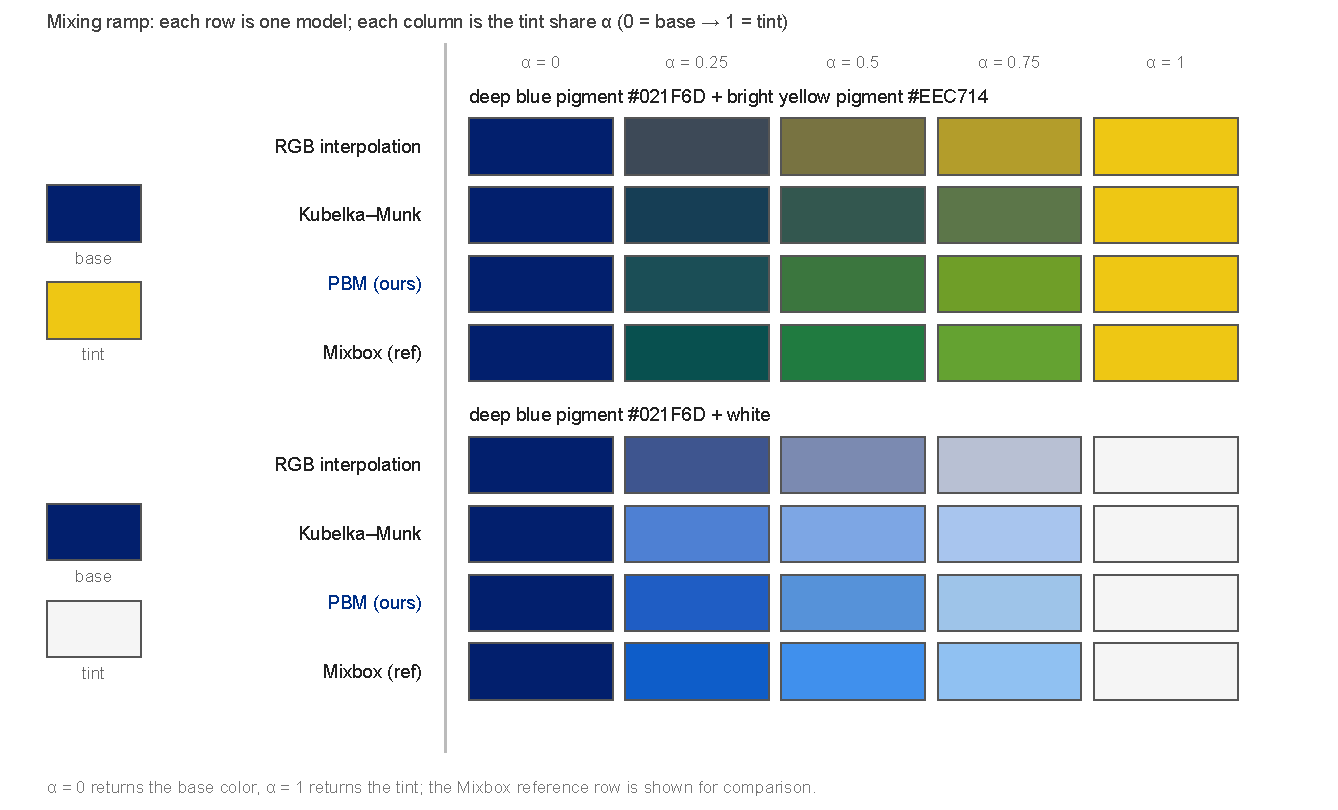
\includegraphics[width=\linewidth]{fig1-mixing.pdf}
\caption{RGB 插值、光谱 K--M、PBM 与 Mixbox 参考的混色行为。上：深蓝颜料与亮黄颜料混合。下：同一深蓝与白混合。每行一个模型；每列为染色占比 $\alpha$（$\alpha=0$ 返回基色，$\alpha=1$ 返回染色）。K--M 行为 \cref{sec:synthetic} 的合成光谱真值：合成颜料光谱经两常数 Duncan 叠加，输入为纯颜料的渲染色。PBM 遵循同样的定性族（黄 $\times$ 蓝 $\rightarrow$ 绿；深 $+$ 白保持色度）。}
\label{fig:overview}
\end{figure}

\section{背景与相关工作}
\label{sec:background}

\subsection{颜料混色的物理}
\label{sec:km}

颜料层的颜色来自颜料颗粒对光的选择性吸收与散射。在 Kubelka--Munk 双流模型中，每种颜料 $i$ 由吸收系数 $K_i(\lambda)$ 与散射系数 $S_i(\lambda)$ 描述。对非负且和为 1 的浓度 $c_i$，Duncan 叠加给出
\begin{equation}
K(\lambda)=\sum_i c_i K_i(\lambda),\qquad
S(\lambda)=\sum_i c_i S_i(\lambda),
\label{eq:duncan}
\end{equation}
不透明层在波长 $\lambda$ 处的反射率为
\begin{equation}
\Rinf(\lambda)=1+\kappa(\lambda)-\sqrt{\kappa(\lambda)^{2}+2\kappa(\lambda)},
\qquad \kappa(\lambda)=\frac{K(\lambda)}{S(\lambda)}.
\label{eq:km}
\end{equation}
将反射率与光源、CIE 标准观察者积分，可选地施加 Saunderson 表面修正，再转换为 sRGB，即得到显示颜色 \cite{saunderson1942,haase1992,wyszecki2000}。该模型具有物理解释，但需要光谱数据：一个 RGB 三元组不能确定 $K_i(\lambda)$ 或 $S_i(\lambda)$，且混合两个任意 RGB 颜色需要数值求解颜料浓度，因为 \cref{eq:km} 对 RGB 没有解析逆。

\subsection{相关工作}
\label{sec:related}

\paragraph{RGB 插值。}
线性插值——多数管线中的混合、合成与涂抹都归结于此——建模的是加性光混合。它对光精确，但对互补颜料产生灰色，并使深色向白色去饱和；这正是本文要处理的两个缺陷。

\paragraph{RYB 插值。}
Gossett 与 Chen \cite{gossett2004} 在三维立方体中插值八个手工选择的颜色，使蓝与黄产生绿色。该构造复现了色相偏移的方向，但不能复现颜料的色度行为；本文不评估该模型。

\paragraph{减性与混合模型。}
叠色滤光片模型只考虑吸收、不考虑散射；黄与蓝产生绿色，但结果过暗且色相有偏差。混合减—加公式 \cite{simonot2014} 使结果变亮，但仍保留大部分颜色误差。

\paragraph{数据驱动方法。}
Lu 等 \cite{lu2014} 在预定比例上插值示例颜料混合物。颜料调色板提取 \cite{aharoni2017,tan2019} 与降阶参数化模型 \cite{shugrina2020} 面向作品操作，而不是任意颜色的交互混色。

\paragraph{Mixbox。}
Mixbox \cite{sochorova2021} 将 sRGB 颜色编码为七维潜向量——四个颜料浓度（酞菁蓝、喹吖啶酮品红、汉莎黄、钛白）与三个加性残差——并训练自实测颜料光谱，使潜空间混合保持在 sRGB 色域内。潜向量线性混合，经 $256^{3}$ 编码器与解码器表转换回 RGB。该模型是本文的参考；它是训练得到的、基于查找表的，而非解析的，且参考实现采用非商业许可。

\section{模型}
\label{sec:model}

\subsection{记号与复合结构}
\label{sec:notation}

PBM 作用于 $[0,1]$ 的 sRGB 显示值；不进行线性化、传递函数或颜色空间转换。模型是混色核心与修复层的复合，
\begin{equation}
\mathbf{o}=\clamp\bigl(\mathbf{C}+\mathbf{d},\,0,\,1\bigr),\qquad
\mathbf{C}=\operatorname{Core}(\cb,\ct,\alpha),\qquad
\mathbf{d}=\operatorname{Repair}(\cb,\ct,\alpha,\mathbf{C}),
\label{eq:composition}
\end{equation}
其中 $\cb$ 为基色、$\ct$ 为染色、$\alpha=\clamp(A,0,1)$ 为染色占比：$\alpha=0$ 返回基色，$\alpha=1$ 返回染色。

\begin{figure}[t]
\centering
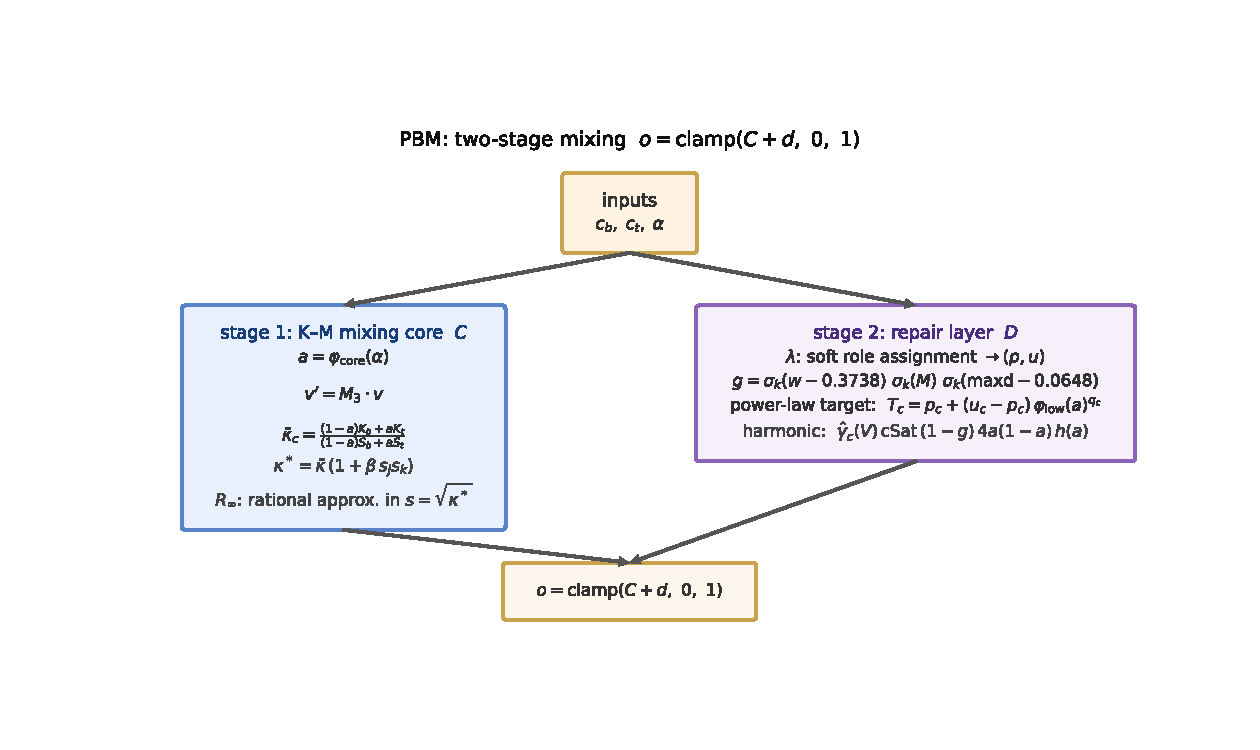
\includegraphics[width=0.82\linewidth]{fig2-architecture.pdf}
\caption{PBM 数据流。两个输入进入 K--M 混色核心（$C$）。修复层分配颜料端与亮端角色（$\lambda$），在门控 $g$ 下计算逐通道幂律目标（$T$），并叠加谐波修正（$\hat{\gamma}$）。修正 $\mathbf{d}$ 加到核心输出后截断。}
\label{fig:architecture}
\end{figure}

修复层对其两个参数的角色是不对称的，而核心是对称的。软角色分配把两种角色次序混合，使完整模型交换对称，
\begin{equation}
F(\cb,\ct,\alpha)\equiv F(\ct,\cb,1-\alpha),
\label{eq:symmetry}
\end{equation}
精确到浮点舍入。

记 $\vp$ 为颜料端、$\vu$ 为亮端（由 \cref{sec:role} 的角色分配选出：最大通道较小的输入扮演颜料）。由 $\vp$ 定义
\begin{equation}
M=\max(\vp),\qquad m=\min(\vp),\qquad \mathrm{maxd}=M-m,\qquad
w=\max\bigl(\min(\vp),\min(\vu)\bigr).
\label{eq:notation}
\end{equation}
斜率为 $k$ 的软阶跃为 $\sigmak(x)=\clamp(kx,0,1)$，$\ssf(x;a,b)$ 表示区间 $[a,b]$ 上的 $C^{1}$ smoothstep。

\subsection{显示值 K/S 混合的结构性缺陷}
\label{sec:defect}

核心在显示值空间中使用解析的吸收与散射默认值进行混合：
\begin{equation}
K(v)=\tfrac12(1-v)^{2},\qquad S(v)=\max(v,\varepsilon),\qquad \varepsilon=0.00157634.
\label{eq:ks-default}
\end{equation}
对白色输入 $v=1$，故 $K=0$、$S=1$；而深色颜料的 $S$ 在 $0.05$--$0.35$ 范围。任意 $\alpha$ 下，白色的散射都主导浓度加权比值的分母，逐通道 $\kappa$ 相互塌缩。

以单通道为例，忽略跨通道矩阵与互吸收修正，考察深蓝 $\#0D1B44=(0.051,0.106,0.267)$ 与白在 $\alpha=0.5$ 时的红通道：
\begin{equation}
\bar{\kappa}_{R}=
\frac{0.5\,K(0.051)+0.5\,K(1)}{0.5\,S(0.051)+0.5\,S(1)}
=\frac{0.5\times0.451}{0.5\times0.051+0.5\times1}=0.429,
\label{eq:defect}
\end{equation}
对应 $\Rinf\approx0.41$。参考 Mixbox 在该通道读出 $0.28$：吸收通道被冲淡。反之蓝通道参考读出 $0.89$，而单通道计算只有 $0.53$：亮化不足。这一失衡是结构性的：白色的 $S=1$ 在任意 $\alpha$ 下都主导混合分母，而加权的 $K$ 与 $S$ 受同一组权重约束，因此在混合阶段重新缩放 $K/S$ 无法恢复被吸收的通道。原始显示值 K--M 叠加在深色加白套件上的平均 $\Delta E_{00}$ 为 10.30（\cref{tab:insample}）。

\subsection{阶段一：K--M 混色核心}
\label{sec:core}

两个输入先经行和为 1 的跨通道矩阵 $\Mthree$ 变换：
\begin{equation}
\mathbf{v}'=\Mthree\mathbf{v},\qquad
\Mthree=
\begin{pmatrix}
0.74523981 & 0.30403013 & -0.04926994\\
0 & 0.74093256 & 0.25906744\\
0 & 0 & 1
\end{pmatrix}.
\label{eq:m3}
\end{equation}
吸收与散射用 \cref{eq:ks-default} 的解析默认值求值。各通道的混合比遵循 Duncan 的浓度结构，并截断到 $[10^{-6},10^{4}]$：
\begin{equation}
\bar{\kappa}_{c}=
\frac{(1-a)\,K(v'_{b,c})+a\,K(v'_{t,c})}
     {(1-a)\,S(v'_{b,c})+a\,S(v'_{t,c})},
\label{eq:kappa}
\end{equation}
其中 $a=\varphi_{\mathrm{core}}(\alpha)$ 为端点压缩后的进度。

逐通道互吸收修正使用另外两个通道 $\{j,k\}$：
\begin{equation}
s'_{c}=\frac{\sqrt{\bar{\kappa}_{c}}}{1+\sqrt{\bar{\kappa}_{c}}},\qquad
\kstar_{c}=\bar{\kappa}_{c}\bigl(1+\beta_{c}\,s'_{j}\,s'_{k}\bigr),\qquad
\beta=(-0.69372345,\,-0.48397409,\,-0.24977842).
\label{eq:beta}
\end{equation}
由于 $s'\in[0,1)$ 且 $\beta_{c}<0$，当其他通道较亮时该修正降低 $\kappa$。

反射率用 $s=\sqrt{\kstar}$ 的有理逼近求值：
\begin{equation}
\Rinf\approx\frac{1}{1+s\bigl(a_{1}+s(a_{2}+s\,a_{3})\bigr)},\qquad
(a_{1},a_{2},a_{3})=\Bigl(\sqrt{2},\,1,\,\tfrac{1}{2\sqrt{2}}\Bigr),
\label{eq:rational}
\end{equation}
该式与 $\Rinf$ 在 $s=0$ 处的前四阶 Taylor 系数一致。在截断范围 $\kstar\in[10^{-6},10^{4}]$ 内，\cref{eq:rational} 的最大绝对误差为 $8.1\times10^{-3}$（在 $\kstar\approx8.1$ 处）；$\kstar\le1$ 时为 $2.5\times10^{-3}$。输出经反变换并截断：
\begin{equation}
\mathbf{C}=\clamp\bigl(\Mthree^{-1}\,\Rinf(\boldsymbol{\kstar}),\,0,\,1\bigr).
\label{eq:core-output}
\end{equation}

\paragraph{动态进度.}
参考在 $\alpha\to1$ 时比显示值 $\kappa$ 混合收敛更快。对 $\alpha=0.99$ 反解参考表明，幂律目标需要的等效进度约为 $10^{-3}$（\cref{sec:inversion}），即 99\% 的混合表现得像 99.9\%。我们用一个作用于核心混合比的对称端点压缩映射来编码这一点：
\begin{equation}
\varphi_{\mathrm{low}}(x)=
\begin{cases}
x, & x\ge w_{\varphi},\\[2pt]
\bigl(1-\ssf(x;0,w_{\varphi})\bigr)x^{p_{\varphi}}+\ssf(x;0,w_{\varphi})\,x, & x<w_{\varphi},
\end{cases}
\label{eq:philow}
\end{equation}
\begin{equation}
\varphi_{\mathrm{core}}(x)=
\begin{cases}
\varphi_{\mathrm{low}}(x), & x<0.5,\\
1-\varphi_{\mathrm{low}}(1-x), & x\ge0.5,
\end{cases}
\label{eq:phicore}
\end{equation}
其中 $p_{\varphi}=1.96522814$、$w_{\varphi}=0.08$。该映射 $C^{1}$ 且关于 $x=0.5$ 反对称，因此核心保持交换对称；当 $x\ge w_{\varphi}$ 时 $\varphi_{\mathrm{low}}(x)=x$，故只影响两端尾部。

\subsection{阶段二：修复层}
\label{sec:repair}

修复层计算加到核心输出上的修正 $\mathbf{d}$，由角色分配、门控、逐通道幂律目标与加性谐波修正组成。

\paragraph{软角色分配.}
\label{sec:role}
颜料端是最大通道较小的输入。硬 argmin 会在 $\max(\cb)=\max(\ct)$ 处不连续切换，故使用软隶属度
\begin{equation}
\lambda=\ssf\!\left(\frac{\max(\ct)-\max(\cb)+E_{W}}{2E_{W}};\,0,\,1\right),
\qquad E_{W}=0.08.
\label{eq:lambda}
\end{equation}
$\lambda=1$ 取 $(\vp,\vu,a)=(\cb,\ct,\alpha)$；$\lambda=0$ 取 $(\ct,\cb,1-\alpha)$；在平局带 $|\max(\ct)-\max(\cb)|<E_{W}$ 内两分支混合：
\begin{equation}
\mathbf{d}=\lambda\,D(\cb,\ct,\alpha)+(1-\lambda)\,D(\ct,\cb,1-\alpha).
\label{eq:dblend}
\end{equation}
带外 $\lambda$ 恰为 $0$ 或 $1$，修复层退化为一次 $D$ 求值。对均匀采样的 sRGB 颜色对，该带约占 $26\%$（在 seed 20260808 的 T3 抽样上实测 26.6\%，在 $2\times10^{5}$ 个均匀对上实测 26.2\%）；因此约四分之三的随机输入会跳过该分支。角色信号取最大通道；也考虑过亮度信号，但它会改变相当比例的随机对的角色判定，故未采用。

\paragraph{深色加亮端门控.}
幂律目标只在深色颜料/亮端区域启用。门控是三个共享斜率 $k=11.0163945$ 的软阶跃之积：
\begin{equation}
g=\sigmak(w-0.37375181)\cdot\sigmak(M)\cdot\sigmak(\mathrm{maxd}-0.06479933).
\label{eq:gate}
\end{equation}
第一个因子在亮端接近消色亮色（$w$ 较大）时开启；第二个在近黑颜料（$M\lesssim1/k\approx0.09$）时压低门控；第三个要求最小色度范围。每个过渡的宽度为 $1/k\approx0.091$，故门控不引入硬截断。对亮色或近消色颜料，$g=0$，直接使用核心输出。

\paragraph{幂律目标.}
在门控区域内，目标遵循从颜料指向亮端的逐通道幂律：
\begin{equation}
T_{c}=p_{c}+(u_{c}-p_{c})\,\varphi_{\mathrm{low}}(a)^{q_{c}}.
\label{eq:target}
\end{equation}
指数 $q_{c}$ 控制通道 $c$ 的亮化速度，由四项组成。

\emph{(a) 软阶跃阶梯.} 在锚点色上反解参考（\cref{sec:inversion}）表明所需指数随通道值 $v$ 下降：暗段保持吸收（高 $q$），亮段快速推进（低 $q$）。该结构由两个阶跃表示：
\begin{equation}
q^{f}(v)=c_{1}^{f}+(c_{2}^{f}-c_{1}^{f})\,\sigmak(v-t_{1})+(c_{3}-c_{2}^{f})\,\sigmak(v-t_{2}),
\qquad f\in\{B,G\},
\label{eq:staircase}
\end{equation}
其中 $t_{1}=0.04350222$、$t_{2}=0.26436295$，系数见 \cref{tab:softstep}。红族为中性，$q^{R}\equiv1$；其通道相关行为由 (d) 的方向响应承担。

\begin{table}[t]
\centering
\small
\caption{亮化指数软阶跃系数（\cref{eq:staircase}）。}
\label{tab:softstep}
\begin{tabular}{lcccc}
\toprule
族 & $c_{1}$（暗） & $c_{2}$（中） & $c_{3}$（亮） & 阶跃位置 / 斜率 \\
\midrule
$B$（蓝，$B$ 最大） & 0.91483121 & 0.32538955 & 0.18785981 & $t_{1}=0.04350222$，$t_{2}=0.26436295$ \\
$G$（绿，$G$ 最大） & 0.57387051 & 0.596528 & 0.18785981 & $k=11.0163945$（共享） \\
$R$（红） & --- & --- & --- & $q^{R}\equiv1$ \\
\bottomrule
\end{tabular}
\end{table}

\emph{(b) 族软混合.} 族权重是颜料通道上的两两支配比较：
\begin{equation}
g_{R}=\tfrac12\,\sigma_{8}(v_{R}-v_{G})+\tfrac12\,\sigma_{8}(v_{R}-v_{B}),
\qquad g_{G}、g_{B}\ \text{同理},
\label{eq:family-weights}
\end{equation}
其中 $\sigma_{8}(x)=\clamp(8x,0,1)$。基础指数为
\begin{equation}
q_{c}^{\mathrm{base}}=\frac{g_{B}q_{c}^{B}+g_{G}q_{c}^{G}+g_{R}q_{c}^{R}}{g_{R}+g_{G}+g_{B}}.
\label{eq:qbase}
\end{equation}
当 $g_{R}+g_{G}+g_{B}<10^{-6}$ 时退化为等权平均，覆盖近灰颜料。

\emph{(c) 通道残差.} 对近零通道，参考曲线依赖通道而非颜料。残差是共享幅度乘以光滑包络：
\begin{equation}
q_{c}\mathrel{+}=\mathrm{RES}_{c}\,e(v_{c}),\qquad
e(v)=
\begin{cases}
A\bigl(1-v/W\bigr)^{2}, & v<W,\\
0, & v\ge W,
\end{cases}
\label{eq:residual}
\end{equation}
其中 $A=0.83421324$、$W=0.14196781$，$\mathrm{RES}=(0,\,-0.24164942,\,-0.24164942)$；红通道残差为零。与分段线性包络不同，\cref{eq:residual} 在 $v=W$ 处 $C^{1}$，且只需三个常数而非八个。

\emph{(d) 通道耦合与方向响应.} 两个通道都高的颜色亮化更慢，且各族的线性方向响应作用在颜料通道上：
\begin{equation}
q_{c}\mathrel{+}=0.42818849\,\sigma_{4.13539205}\Bigl(\max_{i\ne c}v_{i}\Bigr),
\label{eq:coupling}
\end{equation}
\begin{equation}
q_{c}\mathrel{+}=g_{R}\,g^{\mathrm{RTH}}\,\delta^{R}_{c}+g_{B}\,\delta^{B}_{c}+g_{G}\,\delta^{G}_{c},
\qquad
g^{\mathrm{RTH}}=\sigma_{8}(v_{R}-0.21929798),
\label{eq:directional}
\end{equation}
其中
\begin{align}
\delta^{R}&=\bigl[-0.28030789-0.31011215\,v_{R},\nonumber\\
&\qquad 0.33194666-1.19791733\,v_{G},\; -0.45218018+1.71390058\,v_{G}\bigr],\nonumber\\
\delta^{B}&=\bigl[0.40713961,\; -0.08390816+0.76274462\,v_{G},\; 0\bigr],\label{eq:deltas}\\
\delta^{G}&=\bigl[-0.2367074+0.72220875\,v_{R},\; 0,\; -0.30067864+1.03098891\,v_{G}\bigr].\nonumber
\end{align}
范围门 $g^{\mathrm{RTH}}$ 是必要的：线性表达式在 $v_{R}=0.21929798$ 以下改变符号。对两个近黑红 $\#280501$ 与 $\#250903$，在 $\alpha\in[0.1,0.9]$ 上关闭该门会把平均 $\Delta E_{00}$ 从 1.80/2.31 抬到 16.06/13.81（最大值从 2.11/2.66 抬到 18.74/16.45）。

\paragraph{谐波修正.}
在互补色对上反解参考（\cref{sec:inversion}）可看到：混合区间中部的残差呈 $4a(1-a)$ 形状，幅度随输入颜色平滑变化。该修正是在比值特征模板上的线性模型，并在两端衰减：
\begin{equation}
d_{c}\mathrel{+}=\hat{\gamma}_{c}(\vp,\vu)\;\mathrm{cSat}(\vp,\vu)\;(1-g)\;4a(1-a)\;h(a),
\label{eq:harmonic}
\end{equation}
其中
\begin{equation}
\begin{aligned}
h(a)&=\sigma_{14}(0.845-a),\\
\mathrm{cSat}(\vp,\vu)&=\ssf\bigl(\max(\vp)-\min(\vp);0.02,0.15\bigr)\\
&\qquad\cdot\ssf\bigl(\max(\vu)-\min(\vu);0.08,0.30\bigr).
\end{aligned}
\label{eq:csat}
\end{equation}
因子 $(1-g)$ 排除深色加亮端区域。色度衰减 $\mathrm{cSat}$ 在任一端点接近消色轴时把修正压到零。该衰减对连续性很重要：比值特征在零色度附近梯度很大，若去掉 $\mathrm{cSat}$，8 位输入扰动下的最大单步输出变化会从 1.39 升到 2.53 $\Delta E_{00}$（\cref{sec:continuity}）。

幅度是每对颜色计算一次的十七特征模板 $V$ 的线性函数：
\begin{equation}
\hat{\gamma}_{c}(\vp,\vu)=w_{0}^{c}+\sum_{j}w_{j}^{c}\,V_{j},
\label{eq:gamma}
\end{equation}
每通道 17 个系数（共 51 个），由互补族与随机测量的语料上的最小二乘拟合得到（\cref{sec:estimation}）。全部特征都是多项式、通道差值的比值或截断线性式：模板不含三角函数，因此谐波修正只需乘法、加法，以及每个比值一次除法。模板定义见 \cref{tab:features}，系数见 \cref{app:coeff}。与学习的潜表示不同，模板由反解测量手工设计，运行时也不存储任何数据。

\begin{table}[t]
\centering
\scriptsize
\setlength{\tabcolsep}{3pt}
\caption{谐波特征模板（含截距共十七个特征，三通道共用）。全部特征由颜料端 $\vp$ 与亮端 $\vu$ 每对计算一次。}
\label{tab:features}
\begin{tabular}{ll}
\toprule
特征 & 定义 \\
\midrule
截距 & $1$ \\
\texttt{lum} & $0.2126\,p_{R}+0.7152\,p_{G}+0.0722\,p_{B}$ \\
\texttt{lumU} & $0.2126\,u_{R}+0.7152\,u_{G}+0.0722\,u_{B}$ \\
\texttt{pm}、\texttt{pn} & $\max(\vp)$、$\min(\vp)$ \\
\texttt{Mmn} & $\max(\vp)\cdot\min(\vp)$ \\
\texttt{span} & $(\max(\vp)-\min(\vp))(\max(\vu)-\min(\vu))$ \\
\texttt{op} & $1-\tfrac12\bigl[(\max(\vp)-\min(\vp))+(\max(\vu)-\min(\vu))\bigr]$ \\
\texttt{u2} & $u_{B}$ \\
\texttt{dcAbs} & $|u_{R}-p_{R}|$ \\
\texttt{wUcP} & $(u_{R}-u_{B})(p_{B}-p_{R})$ \\
\texttt{dg}、\texttt{ur} & $d_{g}=(p_{G}-p_{B})/\max(M-m,\epsilon)$，$u_{r}=(u_{R}-u_{B})/\max(u_{\max}-u_{\min},\epsilon)$ \\
\texttt{drur}、\texttt{dgug} & $d_{r}u_{r}$、$d_{g}u_{g}$，其中 $d_{r}=(p_{R}-p_{B})/\cdots$、$u_{g}=(u_{G}-u_{B})/\cdots$ \\
\texttt{dcmucm} & $d_{cm}u_{cm}$，其中 $d_{cm}=(p_{R}-p_{G})/\cdots$、$u_{cm}=(u_{R}-u_{G})/\cdots$ \\
\texttt{gRu} & $\tfrac12\sigma_{8}(u_{R}-u_{G})+\tfrac12\sigma_{8}(u_{R}-u_{B})$ \\
\bottomrule
\end{tabular}
\end{table}

\subsection{算法与边界行为}
\label{sec:algorithm}

完整流程见 \cref{alg:pbm}。端点复制步骤按构造使 $\alpha=0$ 与 $\alpha=1$ 精确。其余运算都是连续函数的复合——截断、幂、smoothstep 与线性式——因此模型连续；没有任何分支会让输出值不连续跳变。\Cref{tab:boundary} 汇总边界性质与实测值。

其中 $\operatorname{Core}$ 表示 \cref{eq:phicore,eq:m3,eq:kappa,eq:beta,eq:core-output} 的复合，$D$ 表示 \cref{eq:gate,eq:target,eq:harmonic} 的修复分支。

\begin{algorithm}[t]
\caption{PBM 混色.}
\label{alg:pbm}
\KwIn{基色 $\cb$、染色 $\ct$（$[0,1]$ 的 sRGB 显示值），比例 $A$}
\KwOut{混合色 $\mathbf{o}$}
$\alpha\gets\clamp(A,0,1)$\;
\If{$\alpha=0$}{\Return{$\cb$}}
\If{$\alpha=1$}{\Return{$\ct$}}
$\mathbf{C}\gets\operatorname{Core}(\cb,\ct,\alpha)$\;
$t_{e}\gets\clamp\bigl((\max(\ct)-\max(\cb)+E_{W})/(2E_{W}),0,1\bigr)$\;
\uIf{$t_{e}\le0$}{$\mathbf{d}\gets D(\ct,\cb,1-\alpha,\mathbf{C})$}
\uElseIf{$t_{e}\ge1$}{$\mathbf{d}\gets D(\cb,\ct,\alpha,\mathbf{C})$}
\Else{$\lambda\gets\ssf(t_{e})$;\; $\mathbf{d}\gets\lambda D(\cb,\ct,\alpha,\mathbf{C})+(1-\lambda)D(\ct,\cb,1-\alpha,\mathbf{C})$}
\Return{$\clamp(\mathbf{C}+\mathbf{d},0,1)$}\;
\end{algorithm}

\begin{table}[t]
\centering
\small
\caption{PBM 的边界行为。}
\label{tab:boundary}
\begin{tabular}{p{0.28\linewidth}p{0.64\linewidth}}
\toprule
性质 & 保证 \\
\midrule
$\alpha=0,1$ & 精确返回输入（T4 最大通道误差 0.00000）。 \\
门控之外 & $g=0$：核心输出加谐波修正；门控之内：幂律目标加谐波修正；过渡连续。 \\
连续性 & 连续函数的复合；8 位扰动下实测最大单步 $\Delta E_{00}$ 为 1.388，超过 1.53 的次数为零。 \\
交换对称 & $F(\cb,\ct,\alpha)\equiv F(\ct,\cb,1-\alpha)$；在 5000 个随机对上实测最大 RGB 差 $6.7\times10^{-16}$（seed 20260808）。 \\
\bottomrule
\end{tabular}
\end{table}

\paragraph{复杂度与实现.}
模型执行固定数量的算术运算：两个输入矩阵—向量乘、一个输出矩阵—向量乘、六次平方根、至多五次幂运算，且不含三角函数与对数。它没有数据循环、查找表或迭代，时间与空间复杂度为 $O(1)$。参考实现提供四种语言（JavaScript、Python、Java、C++），常数完全一致；对 2000 个随机对的跨语言测试测得最大 RGB 通道差为 $5\times10^{-10}$，与测试使用的九位小数序列化及初等函数的库级差异一致。

模型的常数在实现中冻结。修改它们需要重跑估计流程与跨语言一致性测试；四个端口在数值字面量层面保持一致。

\section{参数估计}
\label{sec:estimation}

\subsection{参考与度量}
\label{sec:reference}

全部常数都拟合自或反解自公开的 Mixbox~2.0 API \texttt{lerpFloat} 的输出测量，使用 sRGB 显示值浮点路径。参考从官方分发加载，仅供研究对照。度量为 CIEDE2000 \cite{sharma2005}，取 $k_{L}=k_{C}=k_{H}=1$，并对 Sharma 等的 34 组参考对做了验证（最大绝对偏差 $4.95\times10^{-5}$）。混合在显示值上进行，不做线性化；$\Delta E_{00}$ 在转换为 D65 下的 CIELAB 后计算。

\subsection{反解测量}
\label{sec:inversion}

设计由反解参考的测量驱动，而不是对颜料物理的假设。对每个锚点颜色对，在进度 $\alpha$ 处从参考输出读出幂律轨迹所需的逐通道指数：
\begin{equation}
p_{c}(\alpha)=\frac{\ln\bigl((r_{c}-v_{c})/(1-v_{c})\bigr)}{\ln\alpha},
\label{eq:inversion}
\end{equation}
其中 $v_{c}$ 为颜料通道值，$r_{c}$ 为参考输出。

由此得到三点结构观察（支撑数据见 \cref{app:inversion}）。第一，反解指数在 $\alpha$ 上近似恒定：各族在 $\alpha\in[0.1,0.9]$ 上的漂移小于 0.2，这支撑单指数模型；$\alpha\to1$ 附近的漂移由 $\varphi$ 映射处理。第二，指数随通道值呈两级下降——暗段保持吸收、亮段快速推进——这是 \cref{eq:staircase} 的经验依据。第三，残差结构依赖族与通道：近零通道依赖通道而非颜料；红族颜料亮化时保持其绿吸收；互补混合在区间中部留下近似 $4a(1-a)$ 形状的残差。这些观察引出 \cref{sec:repair} 的残差、耦合、方向与谐波项。

\Cref{fig:staircase} 绘出 $\alpha=0.5$ 处的反解指数、软阶跃近似，以及 PBM 输出的端到端反解。

\begin{figure}[t]
\centering
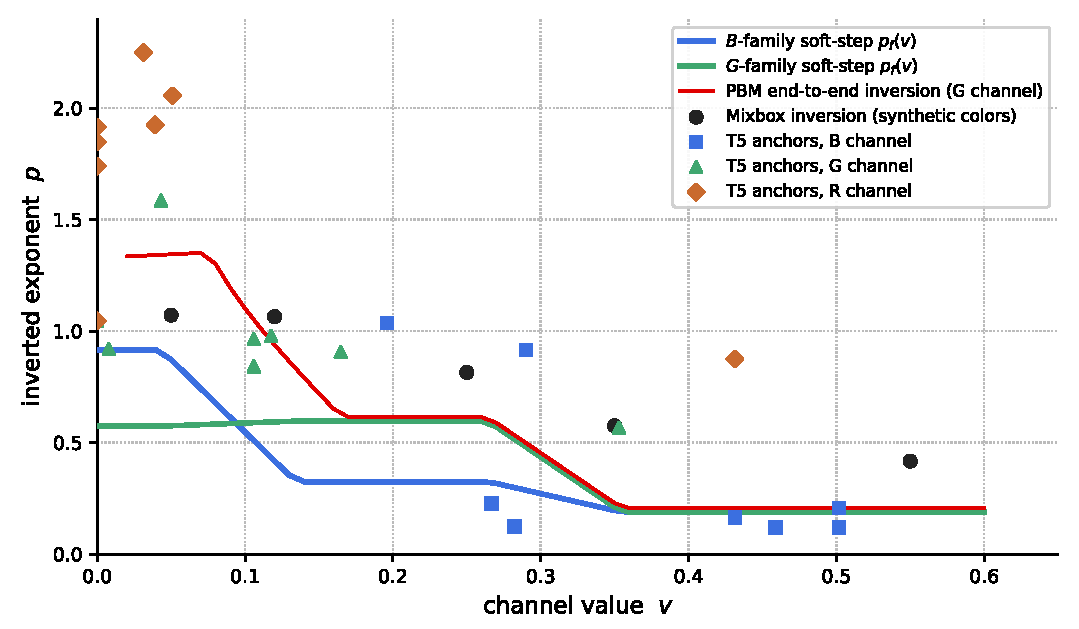
\includegraphics[width=0.78\linewidth]{fig3-staircase.pdf}
\caption{$\alpha=0.5$ 处的反解指数 $p$ 随通道值 $v$ 的变化。点：合成色与 T5 锚点的 Mixbox 反解。线：$B$、$G$ 族的软阶跃近似，以及 PBM 输出的端到端反解（G 通道）。}
\label{fig:staircase}
\end{figure}

\subsection{拟合流程}
\label{sec:fitting}

估计分两阶段，且可由仓库工具完整复现。

\paragraph{语料.}
拟合语料包含调色板套件（T1）、压力对套件（T2）、T3 抽样（seed 20260808）的前 800 个随机对、深色加白套件（T5）、双侧尾端套件（T5E）、6000 个伪随机 sRGB 对（seed 999），以及 12 个锚点互补色对（各取 19 个配比）；锚点对权重为 10，使谐波修正在其起作用处被拟合。

\paragraph{谐波系数.}
由于 $\hat{\gamma}$ 在 \cref{eq:harmonic} 中线性出现，51 个系数可闭式求得。对语料中每个条目，两个角色分支贡献
\begin{equation}
\mathbf{y}=
\mathbf{r}-\mathbf{C}-\sum_{b}\lambda_{b}\,g_{b}\,(T_{b}-\mathbf{C}),
\qquad
\mathbf{A}=\sum_{b}\lambda_{b}\,g_{b}\,V_{b},
\label{eq:design}
\end{equation}
其中 $\mathbf{r}$ 为参考输出，求和遍历当前的一个或两个分支；系数逐通道求解线性最小二乘 $\mathbf{A}\mathbf{w}\approx\mathbf{y}$，岭项取 $10^{-6}$。总增益 $\sum_{b}\lambda_{b}g_{b}$ 低于 0.02 的条目被排除，最终保留 4664 个设计行。

\paragraph{标量.}
其余十四个标量——两个阶梯位置、三个 $B$ 族水平与共享上台阶、耦合幅度与斜率、门控阈值/斜率/色度范围阈值、两个包络常数、端点压缩指数与残差幅度——在样本内损失上由坐标下降精修：
\begin{equation}
L=\overline{\Delta E_{00}}+0.02\,\max\Delta E_{00}+\frac{1}{12}\cdot\overline{\Delta E_{00}}\big|_{\text{锚点}},
\label{eq:loss}
\end{equation}
前两项在 T1、T2、T3 的 800 个拟合对与 T5 上求值。随后做一次交替：在更新后的核心上重拟合谐波系数，各套件变化小于 0.014 $\Delta E_{00}$，即两阶段已到达不动点。拟合得到的常数再在未参与拟合的留出抽样上复核（\cref{sec:results}）。

\paragraph{依测量证据采用的结构简化.}
阶梯斜率并入共享门控斜率；$G$ 与 $B$ 的上台阶共享同一值；$\varphi$ 宽度与 $E_{W}=0.08$ 共享；角色信号取最大通道；残差包络采用 \cref{eq:residual} 的 $C^{1}$ 二次式而非分段线性插值。

\subsection{门控敏感性}
\label{sec:sensitivity}

为检验门控阈值是否被调到狭窄的最优点，在固定其余参数的前提下，把每个门控阈值与共享斜率 $k$ 扰动 $\pm10\%$ 与 $\pm20\%$（\cref{tab:sensitivity}）。T5 的平均 $\Delta E_{00}$ 变化至多 0.11，T3 至多 0.05。T5 均值在 $w_{0}$ 与 $\mathrm{maxd}_{0}$ 扰动下基本不变，在 $k$ 缩放时最多移动 0.11；T3 最大值在 $w_{0}\times0.8$ 时从 19.4 升到 25.2，因为少数互补色对对门控边界敏感。因此这些阈值位于损失的平台上，而非刀刃上。

\begin{table}[t]
\centering
\small
\caption{门控参数敏感性：在固定其余参数时，对每个拟合门控参数施加 $\pm10\%$、$\pm20\%$ 扰动引起的平均 $\Delta E_{00}$ 变化（$\Delta$T5 / $\Delta$T3）。}
\label{tab:sensitivity}
\begin{tabular}{lcccc}
\toprule
参数 & $\times0.8$ & $\times0.9$ & $\times1.1$ & $\times1.2$ \\
\midrule
$w_{0}$（0.37375181） & $+0.000/-0.045$ & $+0.000/-0.023$ & $+0.000/+0.026$ & $+0.000/+0.081$ \\
$\mathrm{maxd}_{0}$（0.06479933） & $-0.011/-0.003$ & $-0.007/-0.002$ & $+0.010/+0.002$ & $+0.025/+0.005$ \\
共享斜率 $k$（11.0163945） & $+0.105/-0.001$ & $+0.029/-0.001$ & $+0.013/+0.002$ & $+0.038/+0.005$ \\
\bottomrule
\end{tabular}
\end{table}

\section{评估}
\label{sec:evaluation}

\subsection{协议}
\label{sec:protocol}

参考为 Mixbox~2.0 \texttt{lerpFloat} 的 sRGB 显示值浮点路径。度量为 CIEDE2000，取 $k_{L}=k_{C}=k_{H}=1$，按 \cref{sec:reference} 所述完成验证。随机集均值给出 bootstrap 95\% 置信区间（1000 次重采样，重采样流固定，故区间可复现）。$\Delta E_{00}$ 的感知刻度只作定性参考：小于 1 接近可察觉阈值，1--2 细看可见，2--4 明显可见，大于 4 为显著差异。

修复层的设计目标为：深色加白套件平均 $\Delta E_{00}$ 低于 5、最大值不超过 15。主套件（T1--T3）不以最大值达标为目标，因为"大变明度差叠加色相对立"的颜色对主导其最大值；我们报告最大值但不将其视为验收标准。

\subsection{测试集与划分}
\label{sec:sets}

\Cref{tab:sets} 汇总测试集；\cref{app:suite} 给出其确切构造、颜色、$\alpha$ 网格与 seed。

\begin{table}[t]
\centering
\footnotesize
\setlength{\tabcolsep}{3pt}
\caption{评估测试集。}
\label{tab:sets}
\begin{tabular}{p{0.16\linewidth}p{0.46\linewidth}rr}
\toprule
集合 & 内容 & $n$ & 角色 \\
\midrule
T1 调色板 & 预设调色板全部对（$10$ 基色 $\times$ $8$ 染色）$\times$ $\alpha\in\{0.25,0.5,0.75\}$ & 240 & 样本内 \\
T2 压力对 & 互补 3、RYB 错配 6、白黑 6、相似 4，各 $\times$ 3 个 $\alpha$ & 57 & 样本内 \\
T3 随机 & 均匀 sRGB 对 $\times$ $\alpha\in[0,1]$，固定 seed & 2000 & 混合 \\
T4 恒等 & 10 个颜色 $\times$ $\alpha\in\{0,1\}$ 自混合 & 20 & 结构 \\
T5 深色+白 & 20 个固定深色 $+$ 24 个随机深色 $\times$ 9 个 $\alpha$ 档 & 396 & 样本内 \\
T5-留出 & 随机深色（新 seed 20260812）$\times$ 9 个 $\alpha$ 档 & 216 & 留出 \\
tail & T5 固定色 $\times$ $\alpha\in[0.92,0.99]$ $+$ 盲区色 $\times$ 全 $\alpha$ & 241 & 样本内 \\
T5E 双侧尾端 & 有色度深色 $\times$ 深重侧 $\alpha$ $+$ 近中性深色 $\times$ 两侧 & 240 & 样本内 \\
\bottomrule
\end{tabular}
\end{table}

拟合语料包含 T1、T2、T5、T5E、tail，以及 T3（seed 20260808）前 800 对。留出数据为不相交的 T3 切片 $[800,2000)$、两个独立 T3 抽样（seed 20260809 与 20260811，与所有拟合 seed 不相交）与 T5-留出（新 seed 20260812）。T3 使用确定性 PRNG（mulberry32），故所有抽样可复现。

T5E 覆盖其他套件稀疏的两侧尾端：20 个有色度深色与 12 个近中性深色在 $\alpha\in\{0.001,\dots,0.1\}$，同 12 个近中性色在 $\alpha\in\{0.92,\dots,0.99\}$。近中性组的色度范围低于门控阈值，因此仅由核心混色；T5E 在该区域监督 $\varphi$ 映射。

\subsection{结果}
\label{sec:results}

\Cref{tab:insample} 报告样本内结果，\cref{tab:heldout} 报告留出结果；\cref{fig:errhist} 给出误差分布。

\begin{table}[t]
\centering
\footnotesize
\setlength{\tabcolsep}{3pt}
\caption{相对 Mixbox~2.0 的样本内结果（$\Delta E_{00}$ 均值 / 最大值）。T3(fit) 为 seed 20260808 抽样的前 800 对。}
\label{tab:insample}
\begin{tabular}{lcccccc}
\toprule
模型 & T1 & T2 & T3(fit) & T5 & tail & T4 \\
\midrule
PBM & \textbf{3.286 / 15.0} & \textbf{2.667 / 10.7} & \textbf{2.759 / 15.5} & \textbf{2.258 / 7.3} & \textbf{1.678 / 8.0} & 0.00000 \\
RGB 插值 & 5.053 / 39.0 & 5.526 / 39.4 & 3.374 / 27.5 & 8.127 / 20.9 & 5.878 / 20.6 & 通过 \\
K--M（显示值） & 4.867 / 27.4 & 5.199 / 25.2 & 3.964 / 23.7 & 10.299 / 23.6 & 9.877 / 24.1 & 通过 \\
\bottomrule
\end{tabular}
\end{table}

\begin{table}[t]
\centering
\footnotesize
\setlength{\tabcolsep}{3pt}
\caption{相对 Mixbox~2.0 的留出结果（$\Delta E_{00}$ 均值 / 最大值；PBM 均值的 bootstrap 95\% 区间见注）。}
\label{tab:heldout}
\begin{tabular}{lcccc}
\toprule
模型 & T3 切片 $[800,2000)$ & T3 seed 09 & T3 seed 11 & T5-留出 \\
\midrule
PBM & \textbf{2.789 / 19.4} & \textbf{2.719 / 23.8} & \textbf{2.852 / 22.2} & \textbf{2.377 / 9.9} \\
RGB 插值 & 3.456 / 36.8 & 3.273 / 34.5 & 3.425 / 34.6 & 7.612 / 17.1 \\
K--M（显示值） & 4.002 / 31.5 & 3.918 / 31.4 & 4.010 / 32.8 & 9.517 / 17.3 \\
\bottomrule
\end{tabular}

\smallskip
{\scriptsize Bootstrap 95\% 置信区间（均值），PBM：切片 [2.662, 2.930]；seed 09 [2.612, 2.834]；seed 11 [2.742, 2.974]；T5-留出 [2.237, 2.540]。}
\end{table}

\begin{figure}[t]
\centering
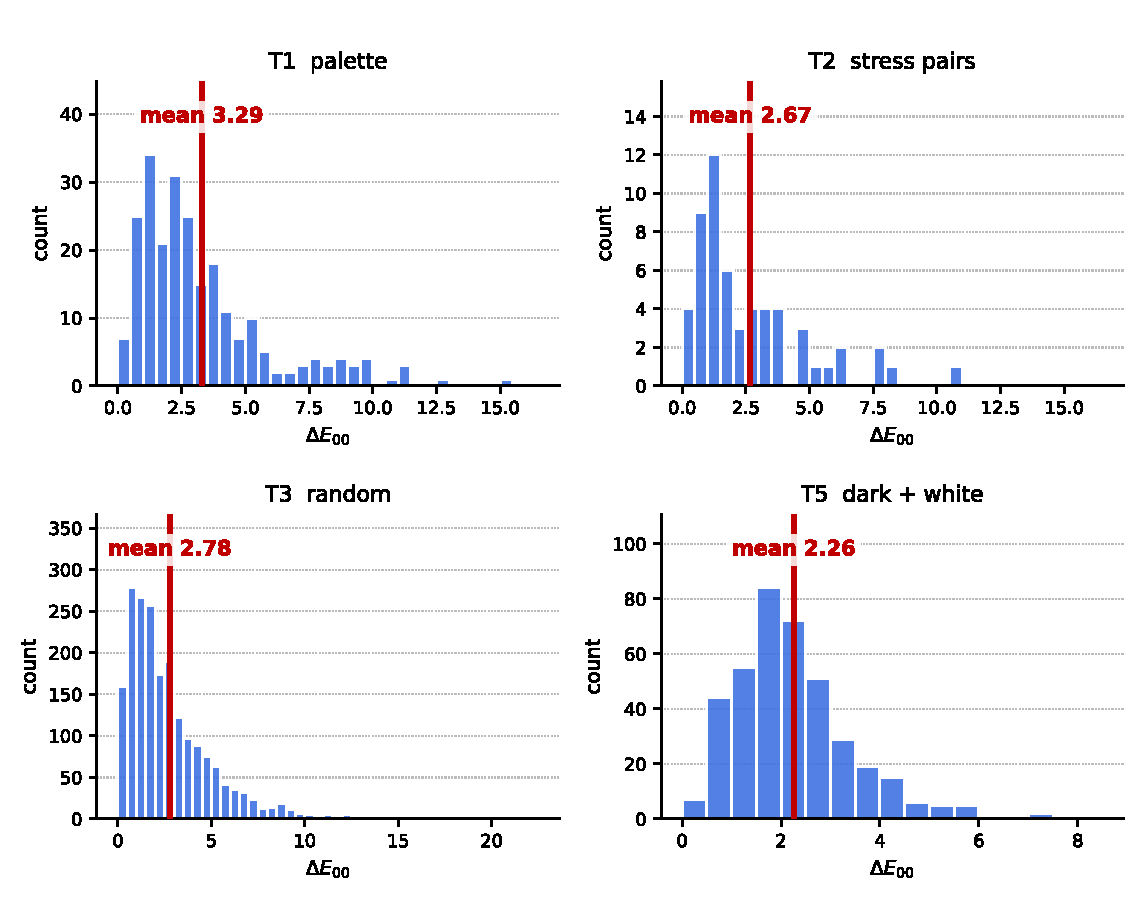
\includegraphics[width=0.72\linewidth]{fig4-error-dist.pdf}
\caption{PBM 相对 Mixbox~2.0 在 T1、T2、T3（seed 20260808，$n=2000$）与 T5 上的 $\Delta E_{00}$ 直方图（组距 0.5；红线为均值）。}
\label{fig:errhist}
\end{figure}

由此得到三点观察。第一，留出均值与拟合抽样相差至多 0.09 $\Delta E_{00}$（T3 切片 2.789 对 2.759），独立抽样（2.719 与 2.852）位于同一区间。在该协议下未发现过拟合证据。第二，留出最大值（19.4--23.8）出现在"大变明度差叠加色相对立"的随机对上；该族是大误差的主要来源（\cref{sec:errors}）。第三，深色加白修复具有泛化性：T5-留出为 2.377，仅比样本内 T5 均值高 0.12，而 RGB 插值（7.61）与原始 K--M（9.52）仍停留在样本内水平。

在 T5E（240 个样本）上，PBM 的均值为 2.441、最大值为 9.5、95 分位为 8.08，位于设计目标之内。$\varphi$ 映射的两次应用都改善了各自针对的颜色对：关闭核心映射使 T5E 均值从 2.441 升到 2.872，关闭幂律目标中的映射使其升到 2.881。

\subsection{消融}
\label{sec:ablation}

\Cref{tab:ablation} 在参考实现中逐项关闭组件。所有变体都由算法源码的文本替换生成，并已验证确实改变了被执行的代码；替换目标缺失时工具会报错。

\begin{table}[t]
\centering
\footnotesize
\setlength{\tabcolsep}{2.5pt}
\caption{消融研究（$\Delta E_{00}$ 均值 / 最大值）。T3 为 seed 20260808 的完整抽样（$n=2000$）。}
\label{tab:ablation}
\begin{tabular}{lccccc}
\toprule
配置 & T1 & T2 & T3 & T5 & tail \\
\midrule
PBM（完整） & \textbf{3.286 / 15.0} & \textbf{2.667 / 10.7} & \textbf{2.777 / 19.4} & \textbf{2.258 / 7.3} & \textbf{1.678 / 8.0} \\
$-$ 跨通道矩阵 $\Mthree$ & 3.674 / 23.8 & 3.534 / 14.9 & 3.218 / 25.6 & 2.259 / 7.3 & 1.678 / 8.0 \\
$-$ 互吸收 $\beta$ & 3.409 / 12.9 & 2.603 / 10.2 & 2.904 / 19.4 & 2.262 / 7.3 & 1.678 / 8.0 \\
$-$ 通道耦合 & 3.797 / 15.0 & 2.978 / 10.7 & 3.857 / 30.9 & 8.834 / 19.7 & 4.670 / 19.7 \\
$-$ 方向响应 & 3.491 / 15.0 & 2.741 / 10.7 & 2.969 / 24.2 & 4.739 / 15.2 & 3.429 / 12.4 \\
$-$ 谐波修正（$\hat{\gamma}$） & 3.649 / 15.3 & 3.543 / 13.5 & 2.890 / 20.0 & 2.258 / 7.3 & 1.678 / 8.0 \\
$-$ 幂律修复（$g\equiv0$） & 3.700 / 15.0 & 3.091 / 10.7 & 3.248 / 20.4 & 9.823 / 23.8 & 8.448 / 24.0 \\
幂律全接管（$g\equiv1$） & 4.785 / 25.2 & 5.237 / 24.4 & 2.967 / 26.1 & 2.248 / 7.3 & 1.654 / 8.0 \\
\bottomrule
\end{tabular}
\end{table}

在深色加白套件上，幂律修复与通道耦合仍是最强的两个贡献项：去掉修复后 T5 从 2.258 升至 9.823，去掉耦合后升至 8.834。耦合在主套件上也是最强的单项（T3 从 2.777 升至 3.857）。跨通道矩阵在主套件上次之（T1 从 3.286 升至 3.674；T2 从 2.667 升至 3.534），在修复主导的 T5 上中性。方向响应在 T5（4.739）与尾端（3.429）上重要。互吸收影响小而混杂：去掉后 T2 变好（2.603）而 T1 变差（3.409），故保留。谐波修正改善全部三个主套件（T1 3.649→3.286；T2 3.543→2.667；T3 2.890→2.777），现为单调有益的组件。强制幂律目标全接管会恶化主套件（T1 4.785、T2 5.237），故门控的区域选择是必要的。

\subsection{误差结构}
\label{sec:errors}

最大误差集中在"大变明度差叠加色相对立"的颜色对上。T1 最差对为近黑 $\#141417$ 与橙 $\#FF7A2A$ 在 $\alpha=0.25$ 处（$\Delta E_{00}=15.02$）；T2 最差对为黄 $\#FFD61A$ 与群青 $\#2E5EFF$ 在 $\alpha=0.75$ 处（10.70）；T3 最差对为浅绿灰 $\#C8D098$ 与蓝紫 $\#3A45E6$ 在 $\alpha\approx0.32$ 处（19.43）。这些混合物中，参考的七维潜空间产生逐通道独立形式无法表示的跨通道关联。在 $\alpha\in[0.05,0.95]$ 上，八个锚点对的平均 $\Delta E_{00}$ 分别为 2.85（黄 $\times$ 深蓝 $\#FFC400+\#000F3D$）、3.16（黄 $\times$ 近边界 $\#FFC400+\#000724$）、5.20（红 $\times$ 绿 $\#A30000+\#00B359$）、7.04（红 $\times$ 青 $\#A30000+\#00D5C0$）、1.79（品红 $\times$ 绿 $\#E33BA8+\#00B359$）、3.80（橙 $\times$ 蓝 $\#FF7A1A+\#2E5EFF$）、9.73（橙 $\times$ 深蓝 $\#FF7A1A+\#001B75$）、5.07（红 $\times$ 深蓝 $\#A30000+\#001B75$）；去掉谐波修正后误差显著增大（\cref{tab:ablation}）。

在 T5 上，最差的固定色对是深紫 $\#080248$ 与白在 $\alpha=0.4$ 处（$\Delta E_{00}=7.3$），随机深色的最坏情况同为 7.3。T5 中的两个近黑红（$\#280501$ 与 $\#250903$）在带范围门时于 $\alpha\in[0.1,0.9]$ 上测得均值 1.80 / 2.31、最大值 2.11 / 2.66；关闭该门会把这些值抬到 16.06 / 13.81 与 18.74 / 16.45。\Cref{fig:white,fig:worst} 给出深色加白的轨迹与最差对。

\begin{figure}[t]
\centering
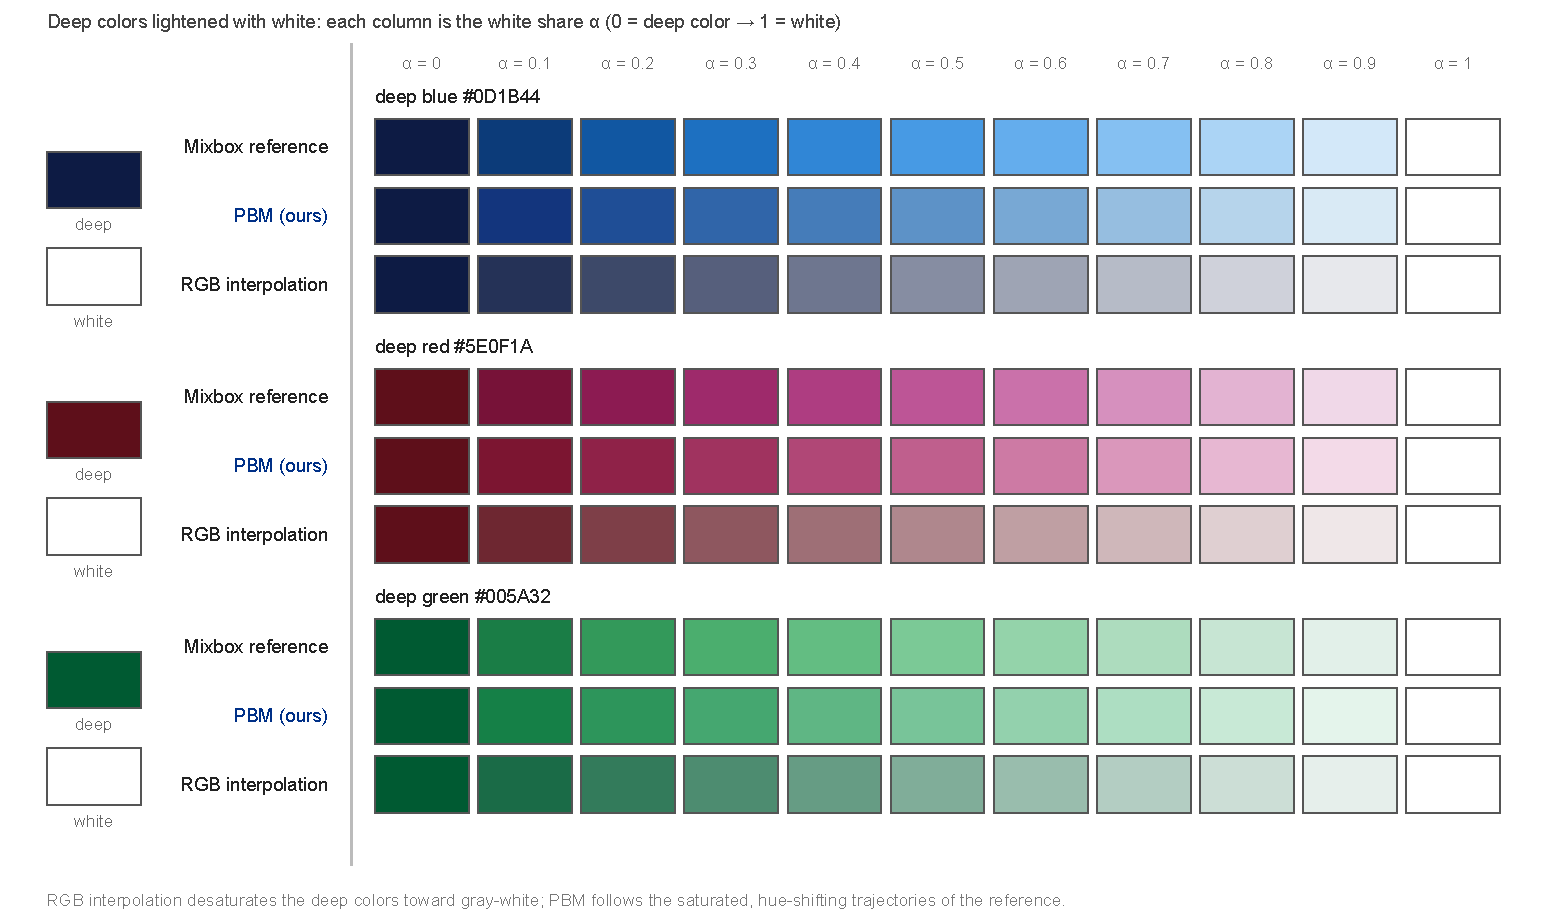
\includegraphics[width=\linewidth]{fig7-mixing-white.pdf}
\caption{深色加白。每列为白色占比 $\alpha$（$0$ = 深色，$1$ = 白）。RGB 插值朝灰白去饱和；PBM 跟随参考的有色度、有色相偏移的轨迹。}
\label{fig:white}
\end{figure}

\begin{figure}[t]
\centering
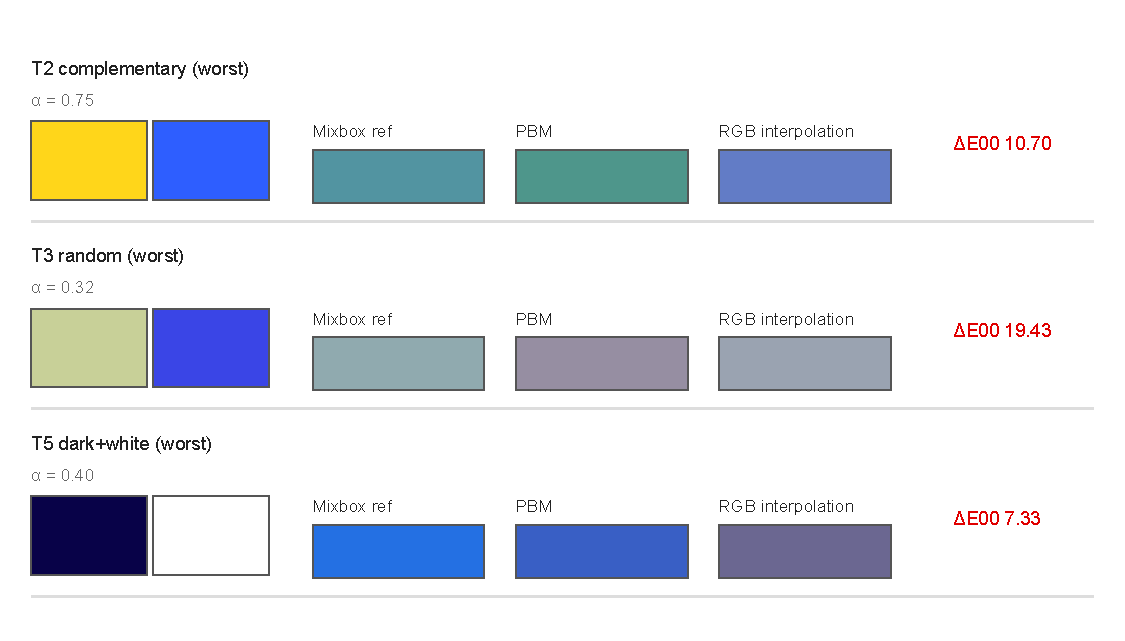
\includegraphics[width=0.82\linewidth]{fig5-worst-pairs.pdf}
\caption{T2 互补、T3 随机与 T5 深色加白套件的最差对：输入、Mixbox 参考输出、PBM 输出、RGB 插值输出，以及 $\Delta E_{00}$。}
\label{fig:worst}
\end{figure}

\subsection{连续性与交换对称}
\label{sec:continuity}

连续性探针对 4000 个随机对的每个输入通道施加 $\pm1/255$ 扰动、对比例施加 $+0.004$，记录输出的最大 $\Delta E_{00}$ 变化。最大单步变化为 1.388，超过 1.53 的次数为零。色度衰减对该结果必要：当 $\mathrm{cSat}\equiv1$ 时，同一探针测得 2.531 与 14 次超阈，原因是比值特征在消色轴附近梯度很大。\Cref{fig:continuity} 给出一个深蓝/白混合的响应。

交换对称在 5000 个随机对（seed 20260808）上测得。$F(\cb,\ct,\alpha)$ 与 $F(\ct,\cb,1-\alpha)$ 的最大 RGB 差为 $6.7\times10^{-16}$，即两分支乘法次序不同带来的浮点舍入。

\begin{figure}[t]
\centering
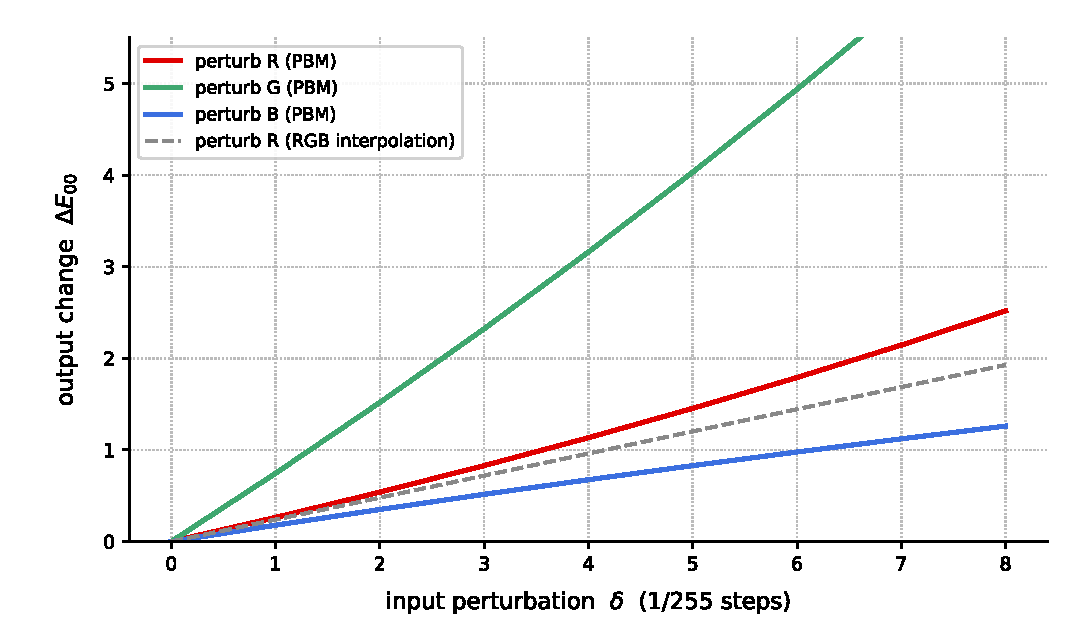
\includegraphics[width=0.72\linewidth]{fig6-continuity.pdf}
\caption{邻域连续性：输出变化 $\Delta E_{00}$ 随输入扰动的变化（对深蓝 $\#0D1B44$ 的每个通道以 1/255 步进，与白在 $\alpha=0.5$ 混合）；虚线为 RGB 插值的响应。}
\label{fig:continuity}
\end{figure}

\subsection{运行时间}
\label{sec:runtime}

\Cref{tab:runtime} 报告在 Windows~11、AMD Ryzen~5 5600X 上使用 Node.js 26.13.1 测得的单次混色时间。全部模型都在宿主 V8 上下文中加载：同一段代码若在 \texttt{node:vm} 沙箱内运行，初等函数调用（\texttt{Math.sqrt}、\texttt{Math.pow}）会被放大一到两个数量级——实测 PBM 为 $8.9\times$、参考为 $8.7\times$——从而扭曲与纯算术基准的对比。PBM、Mixbox 与 RGB 插值使用 $10^{5}$ 个确定性对、预热后九次重复取最好值；光谱 K--M 路径使用 50 对子集，因为迭代反解主导其运行时间。绝对时间依赖于机器与实现；表中比值在同一环境中测得，用于支持接口论证，而不是一般性的性能声明。

\begin{table}[t]
\centering
\small
\caption{单次混色的运行时间（预热后九次重复取最好值）。最后一列为相对 PBM 的时间比。}
\label{tab:runtime}
\begin{tabular}{llrrr}
\toprule
模型 & 路径 & ns/op & ops/s & 相对时间 \\
\midrule
PBM & 解析浮点运算 & 226 & 4{,}431{,}819 & 1.00 \\
Mixbox 2.0 & $256^{3}$ 查找表 & 166 & 6{,}021{,}376 & 0.73 \\
RGB 插值 & 线性混合 & 16 & 63{,}572{,}791 & 0.070 \\
K--M 光谱，直接 & 逐波长 K/S $+$ D65$\times$CMF & 1{,}195 & 836{,}820 & 5.3 \\
K--M 光谱，RGB 输入 & 迭代 unmix $+$ 光谱混合 & 22{,}400{,}000 & 45 & $9.9\times10^{4}$ \\
\bottomrule
\end{tabular}
\end{table}

PBM 的单次成本约为 0.23 $\mu$s，是参考查找表的 1.4 倍、线性混合的 14 倍。光谱 K--M 前向管线本身并不慢：已知颜料光谱时，逐波长积分约需 1.2 $\mu$s，约为 PBM 的 5 倍。障碍在接口：混合两个任意 RGB 颜色需要先把每个颜色反解为颜料浓度，这一迭代优化约需 22 ms，约为 PBM 的 $10^{5}$ 倍。因此 PBM 的优势不是原始速度，而是不需要光谱表示、反解或数兆字节的表。交互绘画中混色按笔触或操作应用，而不是按渲染像素；逐像素渲染时两种模型都会向量化或在 GPU 上实现，此时解析形式更易移植。谐波修正中不含三角函数与对数求值，也使其更易于向量化。

\subsection{相对独立合成光谱世界的验证}
\label{sec:synthetic}

上一节的评估把 PBM 与参考对比。本节改用由合成颜料光谱计算的真值交叉验证，这些光谱未参与 PBM 的拟合。

\paragraph{数据集.}
数据集包含 29 个颜料：覆盖色相环与中性阶的 24 个功能色相，以及用于深色加白套件的 5 个深色派生。每个颜料在 380--750 nm 的 10 nm 网格（38 个采样）上以独立的吸收与散射系数表示：
\begin{equation}
K(\lambda)=\kappa_{\mathrm{base}}+\sum_{i}A_{i}e^{-((\lambda-\mu_{i})/\sigma_{i})^{2}}
+\sum_{j}\frac{B_{j}}{1+e^{\pm((\lambda-\lambda_{j})/w_{j})}},
\qquad S(\lambda)=S_{\mathrm{base}}.
\label{eq:synthetic}
\end{equation}
带位置由第一性原理颜料化学固定（黄/橙/红族的蓝—绿陡吸收边、蓝/绿族的红侧上升边、品红的绿区带、以及过渡金属或有机特征带），幅度、宽度、基底与散射由坐标下降标定到公开的 BabelColor X-Rite ColorChecker Classic Avg30 光谱 \cite{pascale2012}（拟合 $\Delta E_{00}\le1.2$，多数色卡 $\le0.2$）。这些色卡是配方色卡光谱而非纯颜料厚涂光谱；K--M 方程对任意反射率光谱封闭，且色卡面向 RGB 显示设计，故无需显示标定。合成世界是近似，不是实测颜料。

\paragraph{管线与套件.}
前向管线分别叠加 $K$ 与 $S$，逐波长求 \cref{eq:km}，在 10 nm 网格上对 D65 与 CIE 1931 $2^{\circ}$ 观察者积分，再转为 sRGB（截断并标记色域外样本）。所有被比较模型的输入都是纯颜料的渲染 sRGB 颜色，从而避开"某些颜色无法由颜料混出"的问题。六个套件对应 T 套件结构：P1（24 色相调色板全部 828 对）、P2（9 个压力对）、P3（2000 个随机颜料对，新 seed 20260813）、P5（15 个深色颜料 $\times$ 白）、P5-buff（同一深色集 $\times$ 米色）、P5E（双侧尾端网格）。色域外样本被截断并计数。

\Cref{tab:synthetic} 报告结果，\cref{fig:physical} 展示三个代表颜色对。

\begin{table}[t]
\centering
\footnotesize
\setlength{\tabcolsep}{3pt}
\caption{相对合成光谱参考的 $\Delta E_{00}$（均值 / 最大值；随机集均值的 bootstrap 95\% 区间见注；色域外样本截断并计数）。}
\label{tab:synthetic}
\begin{tabular}{lcccccc}
\toprule
模型 & P1 & P2 & P3 & P5 & P5-buff & P5E \\
 & {\scriptsize$n{=}828$, 域外 6} & {\scriptsize$n{=}27$} & {\scriptsize$n{=}2000$, 域外 35} & {\scriptsize$n{=}135$} & {\scriptsize$n{=}135$, 域外 2} & {\scriptsize$n{=}150$, 域外 6} \\
\midrule
PBM & 6.70 / 36.3 & 13.38 / 29.7 & 5.60 / 35.9 & 8.44 / 22.3 & 4.99 / 17.1 & 3.40 / 13.9 \\
Mixbox 2.0 & 6.46 / 31.5 & 12.71 / 24.9 & 5.10 / 30.2 & 8.86 / 25.0 & 4.56 / 18.9 & 3.39 / 20.9 \\
RGB 插值 & 6.14 / 29.5 & 11.25 / 20.4 & 4.89 / 25.4 & 8.24 / 27.0 & 5.95 / 15.8 & 3.88 / 26.9 \\
K--M 显示值 & 5.55 / 30.5 & 8.82 / 16.6 & 4.38 / 30.5 & 12.13 / 30.8 & 4.95 / 18.1 & 4.25 / 28.2 \\
\bottomrule
\end{tabular}

\smallskip
{\scriptsize Bootstrap 95\% 置信区间（均值）：PBM P1 [6.320, 7.045]、P3 [5.390, 5.822]、P5 [7.610, 9.258]；Mixbox P1 [6.080, 6.808]、P3 [4.884, 5.333]、P5 [7.964, 9.786]。}
\end{table}

\begin{figure}[t]
\centering
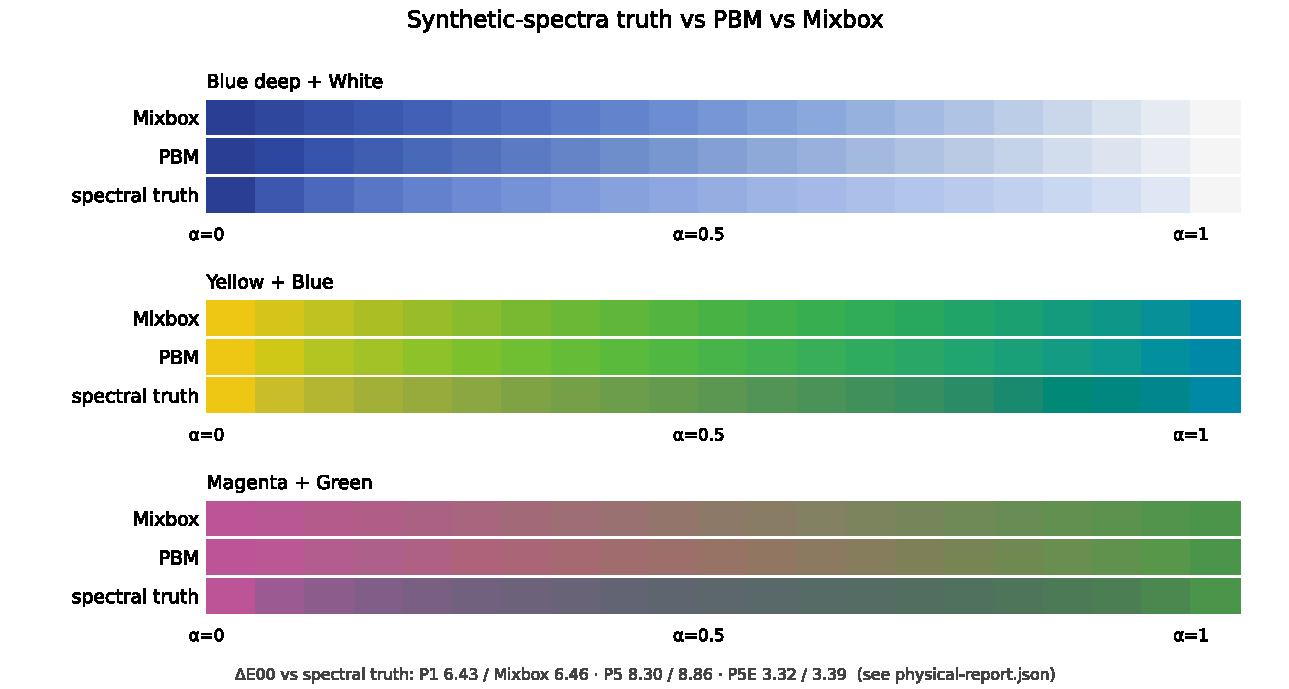
\includegraphics[width=0.88\linewidth]{fig8-physical.pdf}
\caption{合成光谱真值 versus PBM 与 Mixbox：三个代表颜料对（深蓝 $\times$ 白、黄 $\times$ 蓝、品红 $\times$ 绿）在 $\alpha=0$--$1$ 上（21 步）。}
\label{fig:physical}
\end{figure}

由此得到三点观察。第一，PBM 与参考在该世界上相当：各套件均值差 $\mathrm{PBM}-\mathrm{Mixbox}$ 在 $-0.42$（P5）到 $+0.67$（P2）之间，且每对 bootstrap 区间重叠。两者都未在该世界上训练，因此这种平价是 PBM 的精度并非拟合参考输出所致伪影的证据。PBM 在 P5 与 P5E 上更接近真值，参考在 P1、P2、P3、P5-buff 上更接近；本文未检验这些差异的显著性。第二，色相轨迹一致：\cref{tab:hue} 报告有色度样本（$C^{\ast}>10$）的平均与中位绝对色相差。PBM 的平均色相误差在六个套件中的三个（P5、P5-buff、P5E）更低，其余相差在 $2^{\circ}$ 以内。第三，各套件剩余平均误差（3.40--13.38 $\Delta E_{00}$）是结构性的：合成世界按光谱 K--M 混色，而 Mixbox 在训练的潜空间多项式上混色。

\begin{table}[t]
\centering
\small
\caption{与合成光谱真值的色相一致：有色度样本（$C^{\ast}>10$）上平均与中位绝对色相差（度）。}
\label{tab:hue}
\begin{tabular}{lcc}
\toprule
套件 & PBM & Mixbox 2.0 \\
\midrule
P1 & 11.33 / 6.62 & 11.01 / 5.96 \\
P2 & 23.17 / 17.23 & 21.46 / 18.01 \\
P3 & 9.27 / 4.62 & 8.64 / 3.73 \\
P5 & 9.54 / 5.77 & 9.67 / 7.15 \\
P5-buff & 8.59 / 5.79 & 8.62 / 5.30 \\
P5E & 2.56 / 0.62 & 2.73 / 0.74 \\
\bottomrule
\end{tabular}
\end{table}

\paragraph{该实验确立与不确立什么.}
实验支撑两点主张：(i) PBM 的精度不是对参考输出过拟合的伪影，因为它在独立合成光谱世界上与参考相当；(ii) 定性行为族——黄 $\times$ 蓝得绿、互补对得浑浊色、深 $+$ 白保持色相——在两常数光谱 K--M 混色下同样成立。它并不确立 PBM 能预测真实颜料的厚涂混色，也不确立它比参考更接近真实颜料。合成世界本身是近似，PBM 与真实颜料的关系被"参考与真实颜料的关系"加上"PBM 相对参考的实测偏差"共同界定。

\subsection{有效性威胁}
\label{sec:threats}

\paragraph{对参考的依赖.}
PBM 拟合自 Mixbox~2.0。若参考改变，常数必须按 \cref{sec:estimation} 的流程重新估计。实测精度是相对该参考的，并不界定对实测颜料样品的误差。

\paragraph{合成世界.}
交叉验证使用两常数 K--M 混合标定到 ColorChecker 色卡的合成光谱。两常数近似与色卡标定都限制了解释；合成世界不能替代实测颜料光谱。

\paragraph{度量.}
本文使用等权 CIEDE2000。其他色差公式或观察者/光源选择可能改变个别颜色对的排序并影响报告的均值。

\paragraph{抽样.}
固定套件为样本内；只有随机集给出置信区间。置信区间覆盖均值的抽样波动，不覆盖模型选择或实现不确定性。

\paragraph{范围.}
模型定义于 sRGB 显示值空间中不透明、均匀混合的颜色。它不建模分层、罩染、透明度、纹理或光谱输出。

\section{局限与未来工作}
\label{sec:limitations}

\paragraph{残差误差的性质.}
T5 的最大残差（近黑紫，$\Delta E_{00}\approx5.8$）与主套件的最大残差（大变明度差叠加色相对立的颜色对，10.7--23.8）同源：参考在四颜料基上表达其色域，红族与紫色颜料的高阶跨通道关联是该潜表示的性质，不是逐通道独立形式能够表示的。PBM 沿四个维度逼近潜空间行为——K--M 核心、幂律指数、谐波修正与 $\varphi$ 映射——但剩余误差仍主导最大值统计。

\paragraph{近中性深色盲区.}
近中性深色（$\mathrm{maxd}\in[0.02,0.06]$）落在门控之下，仅由核心混色。幂律阶梯是在有色度深色上拟合的，其通道结构与灰调深色所需的近似统一指数不同。残差在浅重侧测得最大值 9.5 $\Delta E_{00}$，T5E 全集中值 2.441。这位于设计目标之内，但在深色加白的设计目标套件（T5、T5E、tail）中是最大的最大值。$\varphi$ 映射减轻但未消除它。

\paragraph{与 Mixbox 的关系.}
Mixbox 采用潜空间线性混合加多项式解码，并在实测颜料光谱上训练。PBM 采用解析 K--M 结构与拟合自参考输出的解析修复层。由于参考的潜空间训练自实测颜料数据，PBM 传递性地继承参考的部分物理合理性；其相对真实颜料的误差被参考自身误差加上 PBM 相对参考的实测偏差所界定。该偏差是完全解析、无需训练表或许可限制的实现代价。

\paragraph{尚存的局限.}
\begin{enumerate}
\item 逐通道独立结构无法表示参考的高阶跨通道关联；这是最大误差的来源。
\item 常数拟合自 Mixbox~2.0。若参考改变，常数必须以 \cref{sec:estimation} 的流程重新估计；它们不能迁移到别的参考。
\item 线性方向响应无法用单一单变量形式同时协调品红与深红。T5 中品红成员的均值为 1.91--1.99、最大值为 2.19--2.86；近黑紫 $\#2A0A5E$ 均值 3.93、最大 5.82；深紫 $\#080248$ 为 5.14 / 7.33。
\item 谐波修正是手工特征模板上的线性模型，其残差在参考轨迹关于混合比非单调的颜色对上最大。非线性但仍解析的修正，以及模型侧新增潜通道，留待未来工作。
\item 合成光谱验证确认了模型在与独立两常数 K--M 世界中的平价性与定性族行为。实测量版本需要实测颜料光谱的授权发布。
\end{enumerate}

未来工作包括：扩展当前模板之外的特征结构、为近中性盲区重拟合阶梯、在核心中加入残差（非光谱）潜通道、把模型推广到分层合成，以及在可获得实测颜料数据时按实物重拟合。

\section{结论}
\label{sec:conclusion}

本文描述 PBM：一个作用在 sRGB 显示值空间、参考校准的解析混色模型。模型将 K--M/Duncan 结构的核心与三层连续混合的修复机制结合：针对深色加白的逐通道幂律目标、针对互补色对的加性谐波修正，以及使模型交换对称的软角色分配。谐波修正是十七个比值特征上的线性模型，因此整个模型不含三角函数与对数，只保留算术、幂与平方根。它 $O(1)$、无查找表，在 $\alpha=0$ 与 $\alpha=1$ 处精确返回输入，按构造连续，并在浮点舍入范围内交换对称（实测探针 $6.7\times10^{-16}$）。51 个谐波系数由最小二乘闭式求得，其余 14 个标量由同一损失上的坐标下降求得；全部常数在四种语言端口中逐位一致。

相对 Mixbox~2.0，PBM 在深色加白套件上的平均 $\Delta E_{00}$ 为 2.258（最大 7.3），在留出深色加白对上为 2.377，在留出随机对上为 2.719--2.852，始终低于 RGB 插值与原始 K--M 叠加。相对独立的合成光谱世界，其各套件平均误差与参考相差至多 0.67 $\Delta E_{00}$，bootstrap 区间全部重叠；平均色相误差在六个套件中的三个更低。剩余的大误差（10.7--23.8 $\Delta E_{00}$）集中在"大变明度差叠加色相对立"的颜色对上，以及近中性深色盲区。

模型的实用价值在于它不需要什么：不需要光谱数据、不需要查找表、不需要训练的潜映射、也不需要第三方许可组件。因此它可以替换绘画软件、游戏引擎与网页应用中的线性 RGB 插值，同时复现颜料混色的定性行为——蓝加黄得到绿、互补色对得到浑浊中性色、深色加白仍保持色度。本文的评估把这一主张界定为"与参考以及与合成光谱世界一致"，并未确立与实测颜料一致。


\begin{thebibliography}{99}
\bibitem{kubelka1931} P.~Kubelka and F.~Munk. Ein Beitrag zur Optik der Farbanstriche. \emph{Zeitschrift f\"ur Technische Physik}, 12:593--601, 1931.
\bibitem{duncan1940} D.~R. Duncan. The colour of pigment mixtures. \emph{Proceedings of the Physical Society}, 52:390--400, 1940.
\bibitem{saunderson1942} J.~L. Saunderson. Calculation of the color of pigmented plastics. \emph{Journal of the Optical Society of America}, 32:727--736, 1942.
\bibitem{pointer1980} M.~R. Pointer. The gamut of real surface colours. \emph{Color Research \& Application}, 5(3):145--155, 1980.
\bibitem{haase1992} C.~S. Haase and G.~W. Meyer. Modeling pigmented materials for realistic image synthesis. \emph{ACM Transactions on Graphics}, 11(4):305--335, 1992.
\bibitem{gossett2004} N.~Gossett and B.~Chen. Paint inspired color mixing and compositing for visualization. In \emph{Proceedings of IEEE InfoVis}, pages 113--118, 2004.
\bibitem{sharma2005} G.~Sharma, W.~Wu, and E.~N. Dalal. The CIEDE2000 color-difference formula: implementation notes, supplementary test data, and mathematical observations. \emph{Color Research \& Application}, 30(1):21--30, 2005.
\bibitem{lu2014} J.~Lu, S.~DiVerdi, W.~Chen, C.~Barnes, and A.~Finkelstein. RealPigment: paint compositing by example. In \emph{Proceedings of NPAR}, pages 21--30, 2014.
\bibitem{simonot2014} L.~Simonot and M.~H\'ebert. Between additive and subtractive color mixings: intermediate mixing models. \emph{Journal of the Optical Society of America A}, 31(1):58--66, 2014.
\bibitem{aharoni2017} E.~Aharoni-Mack, Y.~Shambik, and D.~Lischinski. Pigment-based recolorings of watercolor paintings. In \emph{Proceedings of NPAR}, Article~1, 2017.
\bibitem{tan2019} J.~Tan, S.~DiVerdi, J.~Lu, and Y.~Gingold. Pigmento: pigment-based image analysis and editing. \emph{IEEE Transactions on Visualization and Computer Graphics}, 25(9), 2019.
\bibitem{shugrina2020} M.~Shugrina, A.~Kar, S.~Fidler, and K.~Singh. Nonlinear color triads for approximation, learning and direct manipulation of color distributions. \emph{ACM Transactions on Graphics}, 39(4), Article~97, 2020.
\bibitem{sochorova2021} \v{S}.~Sochorov\'a and O.~Jamri\v{s}ka. Practical pigment mixing for digital painting. \emph{ACM Transactions on Graphics}, 40(6), Article~234, 2021.
\bibitem{wyszecki2000} G.~Wyszecki and W.~S. Stiles. \emph{Color Science: Concepts and Methods, Quantitative Data and Formulae}. 2nd edition, John Wiley \& Sons, 2000.
\bibitem{pascale2012} D.~Pascale. The ColorChecker pages: ColorChecker data (averaged spectral measurements of 30 charts). BabelColor, 2012. \url{http://www.babelcolor.com/colorchecker-2.htm}.
\end{thebibliography}

\crefalias{section}{appendix}
\appendix

\section{评估套件规格}
\label{app:suite}

\subsection{参考与度量}
\begin{itemize}
\item 参考：Mixbox~2.0 \texttt{lerpFloat(base, tint, a)}，从官方分发加载；仅供研究对照，不属于算法本身。
\item 只使用浮点路径（$[0,1]$ 的 sRGB 显示值），避免 8 位量化。
\item 度量：CIEDE2000，取 $k_{L}=k_{C}=k_{H}=1$，包含 $G$ 因子、色相角回绕、权重函数 $S_{L},S_{C},S_{H}$ 与旋转项 $R_{T}$。
\item 复刻校验：实现对照 Sharma 等的 34 组参考对验证，最大偏差 $4.95\times10^{-5}$。
\item 置信区间：bootstrap 95\% 百分位区间（1000 次重采样），重采样流固定。
\end{itemize}

\subsection{测试集}
\begin{itemize}
\item T1：调色板全部对（10 个基色 $\times$ 8 个染色）在 $\alpha\in\{0.25,0.5,0.75\}$（240 个样本）。
\item T2：19 个压力对在三个配比下（57 个样本），列于 \cref{tab:t2}。
\item T3：均匀随机 sRGB 对，$\alpha$ 均匀，seed 20260808，$n=2000$（可配置）。
\item T4：10 个颜色在 $\alpha\in\{0,1\}$ 下自混合；通道容差 0.01。
\item T5：20 个固定深色与 24 个随机深色，各在 $\alpha\in\{0.1,0.2,\dots,0.9\}$（396 个样本）。
\item T5-留出：seed 20260812 的 24 个随机深色，同一 $\alpha$ 网格（216 个样本）。
\item tail：20 个 T5 固定色在 $\alpha\in\{0.92,0.93,\dots,0.99\}$（160 个）与 9 个盲区色在 T5 $\alpha$ 网格上（81 个）。
\item T5E：20 个 T5 固定色在深重侧 $\alpha$（120 个）、12 个近中性色在深重侧 $\alpha$（72 个）以及同 12 色在浅重侧 $\alpha$（48 个）。
\end{itemize}

\begin{table}[t]
\centering
\footnotesize
\setlength{\tabcolsep}{3pt}
\caption{T2 压力对。}
\label{tab:t2}
\begin{tabular}{p{0.16\linewidth}p{0.78\linewidth}}
\toprule
类别 & 颜色对 \\
\midrule
互补对（3） & \#E8321F + \#00D5C0；\#FFD61A + \#2E5EFF；\#E33BA8 + \#00B359 \\
RYB 错配（6） & \#E8321F + \#00B359；\#2E5EFF + \#FF7A1A；\#E8321F + \#2E5EFF；\#FFD61A + \#00B359；\#FFD61A + \#00D5C0；\#E33BA8 + \#00D5C0 \\
白黑混合（6） & \#E8321F、\#2E5EFF、\#FFD61A，各 $\times$ \{\#FFFFFF, \#000000\} \\
相似色（4） & \#E8321F + \#FF7A1A；\#FFD61A + \#FF7A1A；\#2E5EFF + \#8A5BE0；\#00B359 + \#00D5C0 \\
\bottomrule
\end{tabular}
\end{table}

\subsection{T5 与 T5E 套件}
\label{app:t5}

\paragraph{T5 固定色.}
\Cref{tab:t5colors} 列出 20 个固定色：10 个痛点色与 10 个家族扩展色。随机深色用拒绝采样直到 $\max(\mathbf{c})\in[0.30,0.60]$、$\min(\mathbf{c})\le0.08$、$\max(\mathbf{c})-\min(\mathbf{c})\ge0.25$；T5 用 seed 20260810，T5-留出用 seed 20260812。

\begin{table}[t]
\centering
\small
\caption{T5 固定深色（sRGB 十六进制与显示值浮点）。}
\label{tab:t5colors}
\begin{tabular}{llll}
\toprule
Hex & 浮点 RGB & Hex & 浮点 RGB \\
\midrule
$\#0D1B44$ & 0.051, 0.106, 0.267 & $\#0A2A6E$ & 0.039, 0.165, 0.431 \\
$\#000080$ & 0.000, 0.000, 0.502 & $\#8E1F0A$ & 0.557, 0.122, 0.039 \\
$\#001B75$ & 0.000, 0.106, 0.459 & $\#005A32$ & 0.000, 0.353, 0.196 \\
$\#001E80$ & 0.000, 0.118, 0.502 & $\#00552B$ & 0.000, 0.333, 0.169 \\
$\#080248$ & 0.031, 0.008, 0.282 & $\#00585E$ & 0.000, 0.345, 0.369 \\
$\#5F1708$ & 0.373, 0.090, 0.031 & $\#2A0A5E$ & 0.165, 0.039, 0.369 \\
$\#5E0F1A$ & 0.369, 0.059, 0.102 & $\#4A0B6E$ & 0.290, 0.043, 0.431 \\
$\#4A3A05$ & 0.290, 0.227, 0.020 & $\#6E0B4A$ & 0.431, 0.043, 0.290 \\
$\#280501$ & 0.157, 0.020, 0.004 & $\#7A3B00$ & 0.478, 0.231, 0.000 \\
$\#250903$ & 0.145, 0.035, 0.012 & $\#6E4A00$ & 0.431, 0.290, 0.000 \\
\bottomrule
\end{tabular}
\end{table}

\paragraph{T5E.}
深重侧 $\alpha$ 取 0.001、0.005、0.01、0.02、0.05、0.1；浅重侧取 0.92、0.95、0.98、0.99。近中性组为 \#000B2E、\#06052E、\#1A0F22、\#0A1A18，外加 seed 20260816 的 8 个随机色（拒绝采样：$\max\in[0.04,0.10]$，色度范围 $\in[0.02,0.06]$）。

\paragraph{tail 盲区色.}
$\#0D1B44$、$\#001B75$、$\#000080$、$\#001E80$、$\#080248$、$\#0A2A6E$、$\#2A0A5E$、$\#060538$、$\#000333$。

\subsection{划分与统计}
\begin{itemize}
\item 拟合抽样：T1、T2、T5、T5E、tail、T3（seed 20260808）前 800 对、6000 个伪随机对（seed 999），以及 12 个锚点互补色对（各 19 个配比）。
\item 留出：同一次抽样的 T3 第 800--1999 对、seed 20260809 与 20260811 的 T3 抽样、T5-留出（seed 20260812）。
\item 对每个模型与集合报告均值、最大值、中位数、95 分位、标准差，以及（随机集）均值的 bootstrap 95\% 区间。
\item 图表由仓库工具从参考实现生成；每个抽样的 seed 在图表说明或本附录中给出。
\end{itemize}

\section{谐波修正系数}
\label{app:coeff}

\cref{eq:gamma} 的 51 个系数按特征顺序列于下（\cref{tab:features}：截距、\texttt{lum}、\texttt{dgug}、\texttt{dcmucm}、\texttt{wUcP}、\texttt{u2}、\texttt{pm}、\texttt{dg}、\texttt{op}、\texttt{span}、\texttt{drur}、\texttt{pn}、\texttt{Mmn}、\texttt{lumU}、\texttt{ur}、\texttt{dcAbs}、\texttt{gRu}）；截距在首位。

\paragraph{R 通道（17 个系数）.}
$-0.24945965$、$-0.00458899$、$0.00415136$、$-0.03758060$、$0.05450570$、$0.09989345$、$0.25226195$、$0.02321094$、$0.15029394$、$0.03230901$、$0.03005819$、$0.34621807$、$-0.57046216$、$-0.00274566$、$0.03208997$、$-0.05313629$、$-0.02941071$。

\paragraph{G 通道（17 个系数）.}
$-0.15650537$、$0.14061150$、$-0.03620353$、$0.03735064$、$0.02174583$、$0.02381613$、$-0.06481304$、$-0.02027288$、$0.13851721$、$0.13327492$、$0.01269829$、$0.03768178$、$-0.05558582$、$0.03768944$、$0.01505410$、$0.02180116$、$-0.01767582$。

\paragraph{B 通道（17 个系数）.}
$0.16757082$、$-0.04373748$、$0.02221282$、$-0.02131140$、$-0.08893948$、$0.05973609$、$-0.09324463$、$-0.00242072$、$-0.11889782$、$-0.08066689$、$-0.01881345$、$-0.40457567$、$0.51586855$、$-0.01855359$、$0.03390971$、$-0.01807147$、$-0.04148750$。

\section{合成光谱数据集}
\label{app:synthetic}

\subsection{数据集}
模型为两常数 K--M，每个颜料在 380--750 nm 的 10 nm 网格（38 个采样）上分别给出吸收与散射：
\begin{equation}
K(\lambda)=\kappa_{\mathrm{base}}+\sum_{i}A_{i}e^{-((\lambda-\mu_{i})/\sigma_{i})^{2}}+\sum_{j}\frac{B_{j}}{1+e^{\pm((\lambda-\lambda_{j})/w_{j})}},
\qquad S(\lambda)=S_{\mathrm{base}}.
\end{equation}
每个参数都是固定常数；数据集由工具确定性复现。带位置依据第一性原理颜料化学：黄、橙、红与土族在蓝—绿区带陡峭 logistic 吸收边（$\lambda_{0}\approx490$--$585$ nm），蓝与绿在红侧带上升边（$\approx610$--$660$ nm），品红与紫在绿区带高斯带（$\approx550$--$580$ nm），过渡金属或有机颜料另加特征带（$\approx430$--$660$ nm）。幅度、宽度、基底与散射由坐标下降标定到 BabelColor X-Rite ColorChecker Classic Avg30 光谱 \cite{pascale2012}（拟合 $\Delta E_{00}\le1.2$，多数色卡 $\le0.2$）。这些色卡是配方色卡光谱而非纯颜料厚涂光谱；K--M 方程对任意反射率光谱都是封闭的，且该色卡面向 RGB 显示设计，故无需显示标定。

数据集包含 29 个颜料：24 个功能色相（白、黑、米色、浅/中/深灰、蓝灰、两黄、两橙、两红、两品红、紫、三蓝、青、两绿、两土色）与 5 个深色派生（深蓝、红、绿、品红、紫），用于 P5 套件。仓库不含任何第三方测量数据；数值参数离线拟合自公开来源，拟合值随文发表。

\subsection{前向管线与验证}
前向管线分别叠加 $K=(1-\alpha)K_{A}+\alpha K_{B}$ 与 $S=(1-\alpha)S_{A}+\alpha S_{B}$，求 $\kappa=K/S$ 与 \cref{eq:km}，在 10 nm 网格上对 D65 与 CIE 1931 $2^{\circ}$ 观察者积分（梯形法，归一化到 $Y=100$），再转为 IEC 61966-2-1 sRGB，并做截断与色域外标记。

数据集由工具自检：全部 29 个颜料满足 $\Rinf\in(0,1)$ 且 $K\ge0$、$S>0$；纯原色的 unmix 重建 $\Delta E_{00}=0.000$；光谱混合在 $\alpha=0,1$ 处恒等；黄 $\times$ 蓝得到绿（$h^{\circ}\in(110,190)$）；品红 $\times$ 绿与红 $\times$ 青得到浑浊色（$C^{\ast}<30$ 与 $<40$）；深 $+$ 白保持色相（$\alpha=0.25$--$0.75$ 上 $|\Delta h|<40^{\circ}$）；每个颜料都落在其族色相窗内。饱和纯颜料可能合法地超出 sRGB 色域；这些样本被标记并在输入模型前截断（P1：6/828；P3：35/2000；P5：0/135）。

\subsection{套件}
\begin{itemize}
\item P1：24 色相调色板的全部 $\binom{24}{2}$ 个对，$\alpha\in\{0.25,0.5,0.75\}$（828 个样本）。
\item P2：九个互补/压力对，同一组配比（27 个样本）。
\item P3：2000 个随机颜料对，$\alpha$ 均匀，seed 20260813。
\item P5：15 个深色颜料 $\times$ 白，$\alpha\in\{0.1,\dots,0.9\}$（135 个样本）。
\item P5-buff：同一深色集 $\times$ 米色，同一网格（135 个样本）。
\item P5E：深色集 $\times$ 白，$\alpha\in\{0.001,0.005,0.01,0.02,0.05,0.1,0.92,0.95,0.98,0.99\}$（150 个样本）。
\end{itemize}

\section{反解测量}
\label{app:inversion}

本附录中的全部数字都在 Mixbox~2.0 参考（浮点路径）上测得。

\subsection{反解幂指数}
对锚点色，按 \cref{eq:inversion} 逐通道反解指数。\Cref{tab:d1} 报告合成锚点色吸收带在 $\alpha\in\{0.1,\dots,0.9\}$ 上的反解指数（反解最大通道）。各族漂移均小于 0.2；$\alpha\to1$ 处的崩坏正是 $\varphi$ 映射处理的范围。

\begin{table}[t]
\centering
\small
\caption{吸收带的反解指数 $p$ 随 $\alpha$ 的变化（实测）。}
\label{tab:d1}
\begin{tabular}{lccccc}
\toprule
族 & $\alpha=0.1$ & $\alpha=0.3$ & $\alpha=0.5$ & $\alpha=0.7$ & $\alpha=0.9$ \\
\midrule
$B$ & 0.97 & 0.97 & 0.98 & 1.00 & 1.03 \\
$R$ & 0.98 & 1.00 & 1.04 & 1.09 & 1.16 \\
$G$ & 1.00 & 1.03 & 1.07 & 1.12 & 1.18 \\
\bottomrule
\end{tabular}
\end{table}

\Cref{tab:d2} 是 $\alpha=0.5$ 处锚点反解表的摘录，其中 $s$ 为通道沿色度方向的位置。对合成色 $(0.01,v,0.01)$，$s=1$ 通道（G 最大）给出 $v=0.05\rightarrow1.07$、$0.12\rightarrow1.06$、$0.25\rightarrow0.81$、$0.35\rightarrow0.58$、$0.55\rightarrow0.42$；快速亮端区仅在 $v>0.25$ 时适用。

\begin{table}[t]
\centering
\small
\caption{锚点反解表（摘录，$\alpha=0.5$）。}
\label{tab:d2}
\begin{tabular}{lccccc}
\toprule
颜色 & 通道 & $v$ & $s$ & $p$ \\
\midrule
$\#0D1B44$ & R & 0.051 & 0.00 & 2.05 \\
$\#0D1B44$ & G & 0.106 & 0.26 & 0.84 \\
$\#0D1B44$ & B & 0.267 & 1.00 & 0.23 \\
$\#080248$ & R & 0.031 & 0.09 & 2.25 \\
$\#080248$ & B & 0.282 & 1.00 & 0.12 \\
$\#4A0B6E$ & B & 0.431 & 1.00 & 0.85 \\
$\#6E0B4A$ & G & 0.043 & 0.00 & 1.59 \\
$\#5F1708$ & R & 0.373 & 1.00 & 0.76 \\
$\#5F1708$ & G & 0.090 & 0.17 & 1.77 \\
$\#5F1708$ & B & 0.031 & 0.00 & 0.90 \\
$\#8E1F0A$ & R & 0.557 & 1.00 & 0.62 \\
$\#005A32$ & G & 0.353 & 1.00 & 0.57 \\
$\#005A32$ & B & 0.196 & 0.56 & 1.04 \\
$\#6E0B4A$ & B & 0.290 & 0.64 & 0.91 \\
\bottomrule
\end{tabular}
\end{table}

\subsection{残差与耦合}
对 $v=0$ 的通道，参考曲线与颜料无关、只依赖通道（例如 $\#000080$ 的 R 与 G 都为零，但参考曲线不同），这引出残差项。拟合中测得的残差约为 1.85（R）、1.0（G）、1.1（B），并随通道值衰减微调。

耦合项通过固定 $B=0.431$、$G=0.043$ 并在 $\alpha=0.5$ 处扫 $R$ 测得（\cref{tab:d3}）。关系是单调的 S 形：紫 $\#4A0B6E$（$R=0.29$）的 $p_{B}=0.85$，而纯蓝（$R\approx0$）的 $p_{B}=0.12$--$0.17$。耦合是对称的：高 $B$ 使 $R$ 变慢（$B$ 从 0 增至 0.431 时 $p_{R}$ 从 1.04 升到 2.02）。

\begin{table}[t]
\centering
\small
\caption{通道耦合：反解 $p_{B}$ 随 $R$ 的变化（实测）。}
\label{tab:d3}
\begin{tabular}{lccccccc}
\toprule
$R$ & 0.03 & 0.06 & 0.10 & 0.15 & 0.20 & 0.25 & 0.30 \\
$p_{B}$ & 0.17 & 0.21 & 0.35 & 0.60 & 0.73 & 0.80 & 0.85 \\
\bottomrule
\end{tabular}
\end{table}

\subsection{方向响应}
逐 $\alpha$ 反解 T5 红主导固定色可保持 $\alpha$ 恒定性（$\sigma<0.1$）；\cref{tab:d4} 报告逐通道需求。出现三个结构信号：红族 G 保持（$\#5E0F1A$ 与 $\#8E1F0A$ 需要 $G\approx1.7$--$1.8$）、黄褐 B 保持（$\#906D00$ 需要 $B\approx1.5$）、红透射（R 需求为 0.62--0.77）。对 11 个红主导固定色的反解残差做最小二乘（三通道同一线性形式 $\delta_{c}=a+k\,v$），得到 \cref{eq:deltas} 的统一响应。范围门 $g_{R}\sigma_{8}(v_{R}-\mathrm{RTH})$（$\mathrm{RTH}=0.21929798$）是必要的，因为方向系数在其下改变符号。

\begin{table}[t]
\centering
\small
\caption{红族反解：逐通道指数需求（实测）。}
\label{tab:d4}
\begin{tabular}{lccc}
\toprule
颜色 & R 需求 & G 需求 & B 需求 \\
\midrule
$\#5E0F1A$ 深红 & 0.77 & 1.78 & 0.89 \\
$\#8E1F0A$ 深红 & 0.62 & 1.71 & 0.88 \\
$\#906D00$ 赭黄 & 0.72 & 0.95 & 1.49 \\
$\#940C7C$ 品红 & 0.99 & 1.31 & 0.98 \\
\bottomrule
\end{tabular}
\end{table}

\subsection{互补族}
在互补色对上反解参考可见族结构化的残差：对每个色相对立族，误差集中在混合区间中部，形状为 $4a(1-a)$，幅度随两个输入颜色平滑变化。例如亮黄 $\times$ 深蓝族的 G 通道误差近零、B 通道误差至多 0.05，而 R 通道误差在 $\alpha\in[0.4,0.9]$ 上按 $4a(1-a)$ 变化、幅度 0.28--0.29。由于参考的潜空间非线性，幅度跨族平滑变化，单一幅值不足；因此谐波修正是十七特征模板上的线性模型，在互补族语料上拟合（权重 10），每通道 17 个系数。端点抑制 $h(a)$ 与色度衰减 $\mathrm{cSat}$ 是结构性而非拟合得到的。


\end{document}